
% Default to the notebook output style

    


% Inherit from the specified cell style.




    
\documentclass[11pt]{article}

    
    
    \usepackage[T1]{fontenc}
    % Nicer default font (+ math font) than Computer Modern for most use cases
    \usepackage{mathpazo}

    % Basic figure setup, for now with no caption control since it's done
    % automatically by Pandoc (which extracts ![](path) syntax from Markdown).
    \usepackage{graphicx}
    % We will generate all images so they have a width \maxwidth. This means
    % that they will get their normal width if they fit onto the page, but
    % are scaled down if they would overflow the margins.
    \makeatletter
    \def\maxwidth{\ifdim\Gin@nat@width>\linewidth\linewidth
    \else\Gin@nat@width\fi}
    \makeatother
    \let\Oldincludegraphics\includegraphics
    % Set max figure width to be 80% of text width, for now hardcoded.
    \renewcommand{\includegraphics}[1]{\Oldincludegraphics[width=.8\maxwidth]{#1}}
    % Ensure that by default, figures have no caption (until we provide a
    % proper Figure object with a Caption API and a way to capture that
    % in the conversion process - todo).
    \usepackage{caption}
    \DeclareCaptionLabelFormat{nolabel}{}
    \captionsetup{labelformat=nolabel}

    \usepackage{adjustbox} % Used to constrain images to a maximum size 
    \usepackage{xcolor} % Allow colors to be defined
    \usepackage{enumerate} % Needed for markdown enumerations to work
    \usepackage{geometry} % Used to adjust the document margins
    \usepackage{amsmath} % Equations
    \usepackage{amssymb} % Equations
    \usepackage{textcomp} % defines textquotesingle
    % Hack from http://tex.stackexchange.com/a/47451/13684:
    \AtBeginDocument{%
        \def\PYZsq{\textquotesingle}% Upright quotes in Pygmentized code
    }
    \usepackage{upquote} % Upright quotes for verbatim code
    \usepackage{eurosym} % defines \euro
    \usepackage[mathletters]{ucs} % Extended unicode (utf-8) support
    \usepackage[utf8x]{inputenc} % Allow utf-8 characters in the tex document
    \usepackage{fancyvrb} % verbatim replacement that allows latex
    \usepackage{grffile} % extends the file name processing of package graphics 
                         % to support a larger range 
    % The hyperref package gives us a pdf with properly built
    % internal navigation ('pdf bookmarks' for the table of contents,
    % internal cross-reference links, web links for URLs, etc.)
    \usepackage{hyperref}
    \usepackage{longtable} % longtable support required by pandoc >1.10
    \usepackage{booktabs}  % table support for pandoc > 1.12.2
    \usepackage[inline]{enumitem} % IRkernel/repr support (it uses the enumerate* environment)
    \usepackage[normalem]{ulem} % ulem is needed to support strikethroughs (\sout)
                                % normalem makes italics be italics, not underlines
    

    
    
    % Colors for the hyperref package
    \definecolor{urlcolor}{rgb}{0,.145,.698}
    \definecolor{linkcolor}{rgb}{.71,0.21,0.01}
    \definecolor{citecolor}{rgb}{.12,.54,.11}

    % ANSI colors
    \definecolor{ansi-black}{HTML}{3E424D}
    \definecolor{ansi-black-intense}{HTML}{282C36}
    \definecolor{ansi-red}{HTML}{E75C58}
    \definecolor{ansi-red-intense}{HTML}{B22B31}
    \definecolor{ansi-green}{HTML}{00A250}
    \definecolor{ansi-green-intense}{HTML}{007427}
    \definecolor{ansi-yellow}{HTML}{DDB62B}
    \definecolor{ansi-yellow-intense}{HTML}{B27D12}
    \definecolor{ansi-blue}{HTML}{208FFB}
    \definecolor{ansi-blue-intense}{HTML}{0065CA}
    \definecolor{ansi-magenta}{HTML}{D160C4}
    \definecolor{ansi-magenta-intense}{HTML}{A03196}
    \definecolor{ansi-cyan}{HTML}{60C6C8}
    \definecolor{ansi-cyan-intense}{HTML}{258F8F}
    \definecolor{ansi-white}{HTML}{C5C1B4}
    \definecolor{ansi-white-intense}{HTML}{A1A6B2}

    % commands and environments needed by pandoc snippets
    % extracted from the output of `pandoc -s`
    \providecommand{\tightlist}{%
      \setlength{\itemsep}{0pt}\setlength{\parskip}{0pt}}
    \DefineVerbatimEnvironment{Highlighting}{Verbatim}{commandchars=\\\{\}}
    % Add ',fontsize=\small' for more characters per line
    \newenvironment{Shaded}{}{}
    \newcommand{\KeywordTok}[1]{\textcolor[rgb]{0.00,0.44,0.13}{\textbf{{#1}}}}
    \newcommand{\DataTypeTok}[1]{\textcolor[rgb]{0.56,0.13,0.00}{{#1}}}
    \newcommand{\DecValTok}[1]{\textcolor[rgb]{0.25,0.63,0.44}{{#1}}}
    \newcommand{\BaseNTok}[1]{\textcolor[rgb]{0.25,0.63,0.44}{{#1}}}
    \newcommand{\FloatTok}[1]{\textcolor[rgb]{0.25,0.63,0.44}{{#1}}}
    \newcommand{\CharTok}[1]{\textcolor[rgb]{0.25,0.44,0.63}{{#1}}}
    \newcommand{\StringTok}[1]{\textcolor[rgb]{0.25,0.44,0.63}{{#1}}}
    \newcommand{\CommentTok}[1]{\textcolor[rgb]{0.38,0.63,0.69}{\textit{{#1}}}}
    \newcommand{\OtherTok}[1]{\textcolor[rgb]{0.00,0.44,0.13}{{#1}}}
    \newcommand{\AlertTok}[1]{\textcolor[rgb]{1.00,0.00,0.00}{\textbf{{#1}}}}
    \newcommand{\FunctionTok}[1]{\textcolor[rgb]{0.02,0.16,0.49}{{#1}}}
    \newcommand{\RegionMarkerTok}[1]{{#1}}
    \newcommand{\ErrorTok}[1]{\textcolor[rgb]{1.00,0.00,0.00}{\textbf{{#1}}}}
    \newcommand{\NormalTok}[1]{{#1}}
    
    % Additional commands for more recent versions of Pandoc
    \newcommand{\ConstantTok}[1]{\textcolor[rgb]{0.53,0.00,0.00}{{#1}}}
    \newcommand{\SpecialCharTok}[1]{\textcolor[rgb]{0.25,0.44,0.63}{{#1}}}
    \newcommand{\VerbatimStringTok}[1]{\textcolor[rgb]{0.25,0.44,0.63}{{#1}}}
    \newcommand{\SpecialStringTok}[1]{\textcolor[rgb]{0.73,0.40,0.53}{{#1}}}
    \newcommand{\ImportTok}[1]{{#1}}
    \newcommand{\DocumentationTok}[1]{\textcolor[rgb]{0.73,0.13,0.13}{\textit{{#1}}}}
    \newcommand{\AnnotationTok}[1]{\textcolor[rgb]{0.38,0.63,0.69}{\textbf{\textit{{#1}}}}}
    \newcommand{\CommentVarTok}[1]{\textcolor[rgb]{0.38,0.63,0.69}{\textbf{\textit{{#1}}}}}
    \newcommand{\VariableTok}[1]{\textcolor[rgb]{0.10,0.09,0.49}{{#1}}}
    \newcommand{\ControlFlowTok}[1]{\textcolor[rgb]{0.00,0.44,0.13}{\textbf{{#1}}}}
    \newcommand{\OperatorTok}[1]{\textcolor[rgb]{0.40,0.40,0.40}{{#1}}}
    \newcommand{\BuiltInTok}[1]{{#1}}
    \newcommand{\ExtensionTok}[1]{{#1}}
    \newcommand{\PreprocessorTok}[1]{\textcolor[rgb]{0.74,0.48,0.00}{{#1}}}
    \newcommand{\AttributeTok}[1]{\textcolor[rgb]{0.49,0.56,0.16}{{#1}}}
    \newcommand{\InformationTok}[1]{\textcolor[rgb]{0.38,0.63,0.69}{\textbf{\textit{{#1}}}}}
    \newcommand{\WarningTok}[1]{\textcolor[rgb]{0.38,0.63,0.69}{\textbf{\textit{{#1}}}}}
    
    
    % Define a nice break command that doesn't care if a line doesn't already
    % exist.
    \def\br{\hspace*{\fill} \\* }
    % Math Jax compatability definitions
    \def\gt{>}
    \def\lt{<}
    % Document parameters
    \title{Show\_test\_results\_notebook}
    
    
    

    % Pygments definitions
    
\makeatletter
\def\PY@reset{\let\PY@it=\relax \let\PY@bf=\relax%
    \let\PY@ul=\relax \let\PY@tc=\relax%
    \let\PY@bc=\relax \let\PY@ff=\relax}
\def\PY@tok#1{\csname PY@tok@#1\endcsname}
\def\PY@toks#1+{\ifx\relax#1\empty\else%
    \PY@tok{#1}\expandafter\PY@toks\fi}
\def\PY@do#1{\PY@bc{\PY@tc{\PY@ul{%
    \PY@it{\PY@bf{\PY@ff{#1}}}}}}}
\def\PY#1#2{\PY@reset\PY@toks#1+\relax+\PY@do{#2}}

\expandafter\def\csname PY@tok@w\endcsname{\def\PY@tc##1{\textcolor[rgb]{0.73,0.73,0.73}{##1}}}
\expandafter\def\csname PY@tok@c\endcsname{\let\PY@it=\textit\def\PY@tc##1{\textcolor[rgb]{0.25,0.50,0.50}{##1}}}
\expandafter\def\csname PY@tok@cp\endcsname{\def\PY@tc##1{\textcolor[rgb]{0.74,0.48,0.00}{##1}}}
\expandafter\def\csname PY@tok@k\endcsname{\let\PY@bf=\textbf\def\PY@tc##1{\textcolor[rgb]{0.00,0.50,0.00}{##1}}}
\expandafter\def\csname PY@tok@kp\endcsname{\def\PY@tc##1{\textcolor[rgb]{0.00,0.50,0.00}{##1}}}
\expandafter\def\csname PY@tok@kt\endcsname{\def\PY@tc##1{\textcolor[rgb]{0.69,0.00,0.25}{##1}}}
\expandafter\def\csname PY@tok@o\endcsname{\def\PY@tc##1{\textcolor[rgb]{0.40,0.40,0.40}{##1}}}
\expandafter\def\csname PY@tok@ow\endcsname{\let\PY@bf=\textbf\def\PY@tc##1{\textcolor[rgb]{0.67,0.13,1.00}{##1}}}
\expandafter\def\csname PY@tok@nb\endcsname{\def\PY@tc##1{\textcolor[rgb]{0.00,0.50,0.00}{##1}}}
\expandafter\def\csname PY@tok@nf\endcsname{\def\PY@tc##1{\textcolor[rgb]{0.00,0.00,1.00}{##1}}}
\expandafter\def\csname PY@tok@nc\endcsname{\let\PY@bf=\textbf\def\PY@tc##1{\textcolor[rgb]{0.00,0.00,1.00}{##1}}}
\expandafter\def\csname PY@tok@nn\endcsname{\let\PY@bf=\textbf\def\PY@tc##1{\textcolor[rgb]{0.00,0.00,1.00}{##1}}}
\expandafter\def\csname PY@tok@ne\endcsname{\let\PY@bf=\textbf\def\PY@tc##1{\textcolor[rgb]{0.82,0.25,0.23}{##1}}}
\expandafter\def\csname PY@tok@nv\endcsname{\def\PY@tc##1{\textcolor[rgb]{0.10,0.09,0.49}{##1}}}
\expandafter\def\csname PY@tok@no\endcsname{\def\PY@tc##1{\textcolor[rgb]{0.53,0.00,0.00}{##1}}}
\expandafter\def\csname PY@tok@nl\endcsname{\def\PY@tc##1{\textcolor[rgb]{0.63,0.63,0.00}{##1}}}
\expandafter\def\csname PY@tok@ni\endcsname{\let\PY@bf=\textbf\def\PY@tc##1{\textcolor[rgb]{0.60,0.60,0.60}{##1}}}
\expandafter\def\csname PY@tok@na\endcsname{\def\PY@tc##1{\textcolor[rgb]{0.49,0.56,0.16}{##1}}}
\expandafter\def\csname PY@tok@nt\endcsname{\let\PY@bf=\textbf\def\PY@tc##1{\textcolor[rgb]{0.00,0.50,0.00}{##1}}}
\expandafter\def\csname PY@tok@nd\endcsname{\def\PY@tc##1{\textcolor[rgb]{0.67,0.13,1.00}{##1}}}
\expandafter\def\csname PY@tok@s\endcsname{\def\PY@tc##1{\textcolor[rgb]{0.73,0.13,0.13}{##1}}}
\expandafter\def\csname PY@tok@sd\endcsname{\let\PY@it=\textit\def\PY@tc##1{\textcolor[rgb]{0.73,0.13,0.13}{##1}}}
\expandafter\def\csname PY@tok@si\endcsname{\let\PY@bf=\textbf\def\PY@tc##1{\textcolor[rgb]{0.73,0.40,0.53}{##1}}}
\expandafter\def\csname PY@tok@se\endcsname{\let\PY@bf=\textbf\def\PY@tc##1{\textcolor[rgb]{0.73,0.40,0.13}{##1}}}
\expandafter\def\csname PY@tok@sr\endcsname{\def\PY@tc##1{\textcolor[rgb]{0.73,0.40,0.53}{##1}}}
\expandafter\def\csname PY@tok@ss\endcsname{\def\PY@tc##1{\textcolor[rgb]{0.10,0.09,0.49}{##1}}}
\expandafter\def\csname PY@tok@sx\endcsname{\def\PY@tc##1{\textcolor[rgb]{0.00,0.50,0.00}{##1}}}
\expandafter\def\csname PY@tok@m\endcsname{\def\PY@tc##1{\textcolor[rgb]{0.40,0.40,0.40}{##1}}}
\expandafter\def\csname PY@tok@gh\endcsname{\let\PY@bf=\textbf\def\PY@tc##1{\textcolor[rgb]{0.00,0.00,0.50}{##1}}}
\expandafter\def\csname PY@tok@gu\endcsname{\let\PY@bf=\textbf\def\PY@tc##1{\textcolor[rgb]{0.50,0.00,0.50}{##1}}}
\expandafter\def\csname PY@tok@gd\endcsname{\def\PY@tc##1{\textcolor[rgb]{0.63,0.00,0.00}{##1}}}
\expandafter\def\csname PY@tok@gi\endcsname{\def\PY@tc##1{\textcolor[rgb]{0.00,0.63,0.00}{##1}}}
\expandafter\def\csname PY@tok@gr\endcsname{\def\PY@tc##1{\textcolor[rgb]{1.00,0.00,0.00}{##1}}}
\expandafter\def\csname PY@tok@ge\endcsname{\let\PY@it=\textit}
\expandafter\def\csname PY@tok@gs\endcsname{\let\PY@bf=\textbf}
\expandafter\def\csname PY@tok@gp\endcsname{\let\PY@bf=\textbf\def\PY@tc##1{\textcolor[rgb]{0.00,0.00,0.50}{##1}}}
\expandafter\def\csname PY@tok@go\endcsname{\def\PY@tc##1{\textcolor[rgb]{0.53,0.53,0.53}{##1}}}
\expandafter\def\csname PY@tok@gt\endcsname{\def\PY@tc##1{\textcolor[rgb]{0.00,0.27,0.87}{##1}}}
\expandafter\def\csname PY@tok@err\endcsname{\def\PY@bc##1{\setlength{\fboxsep}{0pt}\fcolorbox[rgb]{1.00,0.00,0.00}{1,1,1}{\strut ##1}}}
\expandafter\def\csname PY@tok@kc\endcsname{\let\PY@bf=\textbf\def\PY@tc##1{\textcolor[rgb]{0.00,0.50,0.00}{##1}}}
\expandafter\def\csname PY@tok@kd\endcsname{\let\PY@bf=\textbf\def\PY@tc##1{\textcolor[rgb]{0.00,0.50,0.00}{##1}}}
\expandafter\def\csname PY@tok@kn\endcsname{\let\PY@bf=\textbf\def\PY@tc##1{\textcolor[rgb]{0.00,0.50,0.00}{##1}}}
\expandafter\def\csname PY@tok@kr\endcsname{\let\PY@bf=\textbf\def\PY@tc##1{\textcolor[rgb]{0.00,0.50,0.00}{##1}}}
\expandafter\def\csname PY@tok@bp\endcsname{\def\PY@tc##1{\textcolor[rgb]{0.00,0.50,0.00}{##1}}}
\expandafter\def\csname PY@tok@fm\endcsname{\def\PY@tc##1{\textcolor[rgb]{0.00,0.00,1.00}{##1}}}
\expandafter\def\csname PY@tok@vc\endcsname{\def\PY@tc##1{\textcolor[rgb]{0.10,0.09,0.49}{##1}}}
\expandafter\def\csname PY@tok@vg\endcsname{\def\PY@tc##1{\textcolor[rgb]{0.10,0.09,0.49}{##1}}}
\expandafter\def\csname PY@tok@vi\endcsname{\def\PY@tc##1{\textcolor[rgb]{0.10,0.09,0.49}{##1}}}
\expandafter\def\csname PY@tok@vm\endcsname{\def\PY@tc##1{\textcolor[rgb]{0.10,0.09,0.49}{##1}}}
\expandafter\def\csname PY@tok@sa\endcsname{\def\PY@tc##1{\textcolor[rgb]{0.73,0.13,0.13}{##1}}}
\expandafter\def\csname PY@tok@sb\endcsname{\def\PY@tc##1{\textcolor[rgb]{0.73,0.13,0.13}{##1}}}
\expandafter\def\csname PY@tok@sc\endcsname{\def\PY@tc##1{\textcolor[rgb]{0.73,0.13,0.13}{##1}}}
\expandafter\def\csname PY@tok@dl\endcsname{\def\PY@tc##1{\textcolor[rgb]{0.73,0.13,0.13}{##1}}}
\expandafter\def\csname PY@tok@s2\endcsname{\def\PY@tc##1{\textcolor[rgb]{0.73,0.13,0.13}{##1}}}
\expandafter\def\csname PY@tok@sh\endcsname{\def\PY@tc##1{\textcolor[rgb]{0.73,0.13,0.13}{##1}}}
\expandafter\def\csname PY@tok@s1\endcsname{\def\PY@tc##1{\textcolor[rgb]{0.73,0.13,0.13}{##1}}}
\expandafter\def\csname PY@tok@mb\endcsname{\def\PY@tc##1{\textcolor[rgb]{0.40,0.40,0.40}{##1}}}
\expandafter\def\csname PY@tok@mf\endcsname{\def\PY@tc##1{\textcolor[rgb]{0.40,0.40,0.40}{##1}}}
\expandafter\def\csname PY@tok@mh\endcsname{\def\PY@tc##1{\textcolor[rgb]{0.40,0.40,0.40}{##1}}}
\expandafter\def\csname PY@tok@mi\endcsname{\def\PY@tc##1{\textcolor[rgb]{0.40,0.40,0.40}{##1}}}
\expandafter\def\csname PY@tok@il\endcsname{\def\PY@tc##1{\textcolor[rgb]{0.40,0.40,0.40}{##1}}}
\expandafter\def\csname PY@tok@mo\endcsname{\def\PY@tc##1{\textcolor[rgb]{0.40,0.40,0.40}{##1}}}
\expandafter\def\csname PY@tok@ch\endcsname{\let\PY@it=\textit\def\PY@tc##1{\textcolor[rgb]{0.25,0.50,0.50}{##1}}}
\expandafter\def\csname PY@tok@cm\endcsname{\let\PY@it=\textit\def\PY@tc##1{\textcolor[rgb]{0.25,0.50,0.50}{##1}}}
\expandafter\def\csname PY@tok@cpf\endcsname{\let\PY@it=\textit\def\PY@tc##1{\textcolor[rgb]{0.25,0.50,0.50}{##1}}}
\expandafter\def\csname PY@tok@c1\endcsname{\let\PY@it=\textit\def\PY@tc##1{\textcolor[rgb]{0.25,0.50,0.50}{##1}}}
\expandafter\def\csname PY@tok@cs\endcsname{\let\PY@it=\textit\def\PY@tc##1{\textcolor[rgb]{0.25,0.50,0.50}{##1}}}

\def\PYZbs{\char`\\}
\def\PYZus{\char`\_}
\def\PYZob{\char`\{}
\def\PYZcb{\char`\}}
\def\PYZca{\char`\^}
\def\PYZam{\char`\&}
\def\PYZlt{\char`\<}
\def\PYZgt{\char`\>}
\def\PYZsh{\char`\#}
\def\PYZpc{\char`\%}
\def\PYZdl{\char`\$}
\def\PYZhy{\char`\-}
\def\PYZsq{\char`\'}
\def\PYZdq{\char`\"}
\def\PYZti{\char`\~}
% for compatibility with earlier versions
\def\PYZat{@}
\def\PYZlb{[}
\def\PYZrb{]}
\makeatother


    % Exact colors from NB
    \definecolor{incolor}{rgb}{0.0, 0.0, 0.5}
    \definecolor{outcolor}{rgb}{0.545, 0.0, 0.0}



    
    % Prevent overflowing lines due to hard-to-break entities
    \sloppy 
    % Setup hyperref package
    \hypersetup{
      breaklinks=true,  % so long urls are correctly broken across lines
      colorlinks=true,
      urlcolor=urlcolor,
      linkcolor=linkcolor,
      citecolor=citecolor,
      }
    % Slightly bigger margins than the latex defaults
    
    \geometry{verbose,tmargin=1in,bmargin=1in,lmargin=1in,rmargin=1in}
    
    

    \begin{document}
    
    
    \maketitle
    
    

    
    \begin{Verbatim}[commandchars=\\\{\}]
{\color{incolor}In [{\color{incolor}95}]:} \PY{k+kn}{from} \PY{n+nn}{IPython}\PY{n+nn}{.}\PY{n+nn}{display} \PY{k}{import} \PY{n}{HTML}
         
         \PY{n}{HTML}\PY{p}{(}\PY{l+s+s1}{\PYZsq{}\PYZsq{}\PYZsq{}}\PY{l+s+s1}{\PYZlt{}script\PYZgt{}}
         \PY{l+s+s1}{code\PYZus{}show=true; }
         \PY{l+s+s1}{function code\PYZus{}toggle() }\PY{l+s+s1}{\PYZob{}}
         \PY{l+s+s1}{ if (code\PYZus{}show)}\PY{l+s+s1}{\PYZob{}}
         \PY{l+s+s1}{ \PYZdl{}(}\PY{l+s+s1}{\PYZsq{}}\PY{l+s+s1}{div.input}\PY{l+s+s1}{\PYZsq{}}\PY{l+s+s1}{).hide();}
         \PY{l+s+s1}{ \PYZcb{} else }\PY{l+s+s1}{\PYZob{}}
         \PY{l+s+s1}{ \PYZdl{}(}\PY{l+s+s1}{\PYZsq{}}\PY{l+s+s1}{div.input}\PY{l+s+s1}{\PYZsq{}}\PY{l+s+s1}{).show();}
         \PY{l+s+s1}{ \PYZcb{}}
         \PY{l+s+s1}{ code\PYZus{}show = !code\PYZus{}show}
         \PY{l+s+s1}{\PYZcb{} }
         \PY{l+s+s1}{\PYZdl{}( document ).ready(code\PYZus{}toggle);}
         \PY{l+s+s1}{\PYZlt{}/script\PYZgt{}}
         \PY{l+s+s1}{Show/hide the code by clicking here \PYZlt{}a href=}\PY{l+s+s1}{\PYZdq{}}\PY{l+s+s1}{javascript:code\PYZus{}toggle()}\PY{l+s+s1}{\PYZdq{}}\PY{l+s+s1}{\PYZgt{}here\PYZlt{}/a\PYZgt{}.}\PY{l+s+s1}{\PYZsq{}\PYZsq{}\PYZsq{}}\PY{p}{)}
\end{Verbatim}


\begin{Verbatim}[commandchars=\\\{\}]
{\color{outcolor}Out[{\color{outcolor}95}]:} <IPython.core.display.HTML object>
\end{Verbatim}
            
    \begin{Verbatim}[commandchars=\\\{\}]
{\color{incolor}In [{\color{incolor}92}]:} \PY{o}{\PYZpc{}}\PY{k}{matplotlib} inline
         
         \PY{c+c1}{\PYZsh{}\PYZsh{}\PYZsh{}\PYZsh{}\PYZsh{} don\PYZsq{}t show warnings}
         \PY{k+kn}{import} \PY{n+nn}{warnings}
         \PY{n}{warnings}\PY{o}{.}\PY{n}{simplefilter}\PY{p}{(}\PY{n}{action}\PY{o}{=}\PY{l+s+s1}{\PYZsq{}}\PY{l+s+s1}{ignore}\PY{l+s+s1}{\PYZsq{}}\PY{p}{,} \PY{n}{category}\PY{o}{=}\PY{n+ne}{FutureWarning}\PY{p}{)}
         
         \PY{c+c1}{\PYZsh{}\PYZsh{}\PYZsh{}\PYZsh{}\PYZsh{} import packages}
         \PY{k+kn}{from} \PY{n+nn}{brian2} \PY{k}{import} \PY{o}{*}
         \PY{k+kn}{from} \PY{n+nn}{brian2}\PY{n+nn}{.}\PY{n+nn}{units}\PY{n+nn}{.}\PY{n+nn}{constants} \PY{k}{import} \PY{n}{zero\PYZus{}celsius}\PY{p}{,} \PY{n}{gas\PYZus{}constant} \PY{k}{as} \PY{n}{R}\PY{p}{,} \PY{n}{faraday\PYZus{}constant} \PY{k}{as} \PY{n}{F}
         \PY{k+kn}{import} \PY{n+nn}{numpy} \PY{k}{as} \PY{n+nn}{np}
         \PY{k+kn}{import} \PY{n+nn}{pandas} \PY{k}{as} \PY{n+nn}{pd}
         \PY{n}{pd}\PY{o}{.}\PY{n}{set\PYZus{}option}\PY{p}{(}\PY{l+s+s1}{\PYZsq{}}\PY{l+s+s1}{display.width}\PY{l+s+s1}{\PYZsq{}}\PY{p}{,} \PY{l+m+mi}{115}\PY{p}{)}
         \PY{k+kn}{import} \PY{n+nn}{matplotlib}\PY{n+nn}{.}\PY{n+nn}{pyplot} \PY{k}{as} \PY{n+nn}{plt}
         \PY{k+kn}{import} \PY{n+nn}{os}
         \PY{k+kn}{from} \PY{n+nn}{IPython}\PY{n+nn}{.}\PY{n+nn}{display} \PY{k}{import} \PY{n}{Markdown} \PY{k}{as} \PY{n}{md}
         
         \PY{c+c1}{\PYZsh{}\PYZsh{}\PYZsh{}\PYZsh{}\PYZsh{} sets working directory}
         \PY{n}{os}\PY{o}{.}\PY{n}{chdir}\PY{p}{(}\PY{l+s+s2}{\PYZdq{}}\PY{l+s+s2}{C:/Users/Richard/Documents/Studium/Master Elektrotechnik/Semester 4/Python/Models Brian2}\PY{l+s+s2}{\PYZdq{}}\PY{p}{)}
         
         \PY{c+c1}{\PYZsh{}\PYZsh{}\PYZsh{}\PYZsh{}\PYZsh{} import models}
         \PY{k+kn}{import} \PY{n+nn}{models}\PY{n+nn}{.}\PY{n+nn}{Rattay\PYZus{}2001} \PY{k}{as} \PY{n+nn}{rattay\PYZus{}01}
         \PY{k+kn}{import} \PY{n+nn}{models}\PY{n+nn}{.}\PY{n+nn}{Frijns\PYZus{}1994} \PY{k}{as} \PY{n+nn}{frijns\PYZus{}94}
         \PY{k+kn}{import} \PY{n+nn}{models}\PY{n+nn}{.}\PY{n+nn}{Frijns\PYZus{}2005} \PY{k}{as} \PY{n+nn}{frijns\PYZus{}05}
         \PY{k+kn}{import} \PY{n+nn}{models}\PY{n+nn}{.}\PY{n+nn}{Smit\PYZus{}2009} \PY{k}{as} \PY{n+nn}{smit\PYZus{}09}
         \PY{k+kn}{import} \PY{n+nn}{models}\PY{n+nn}{.}\PY{n+nn}{Smit\PYZus{}2010} \PY{k}{as} \PY{n+nn}{smit\PYZus{}10}
         \PY{k+kn}{import} \PY{n+nn}{models}\PY{n+nn}{.}\PY{n+nn}{Imennov\PYZus{}2009} \PY{k}{as} \PY{n+nn}{imennov\PYZus{}09}
         \PY{k+kn}{import} \PY{n+nn}{models}\PY{n+nn}{.}\PY{n+nn}{Negm\PYZus{}2014} \PY{k}{as} \PY{n+nn}{negm\PYZus{}14}
         
         \PY{c+c1}{\PYZsh{}\PYZsh{}\PYZsh{}\PYZsh{}\PYZsh{} makes code faster and prevents warning}
         \PY{n}{prefs}\PY{o}{.}\PY{n}{codegen}\PY{o}{.}\PY{n}{target} \PY{o}{=} \PY{l+s+s2}{\PYZdq{}}\PY{l+s+s2}{numpy}\PY{l+s+s2}{\PYZdq{}}
         
         \PY{c+c1}{\PYZsh{} =============================================================================}
         \PY{c+c1}{\PYZsh{} Load data}
         \PY{c+c1}{\PYZsh{} =============================================================================}
         \PY{c+c1}{\PYZsh{}\PYZsh{}\PYZsh{}\PYZsh{}\PYZsh{} choose model}
         \PY{n}{model} \PY{o}{=} \PY{n}{rattay\PYZus{}01}
         
         \PY{c+c1}{\PYZsh{}\PYZsh{}\PYZsh{}\PYZsh{}\PYZsh{} load datasets}
         \PY{n}{strength\PYZus{}duration\PYZus{}data} \PY{o}{=} \PY{n}{pd}\PY{o}{.}\PY{n}{read\PYZus{}csv}\PY{p}{(}\PY{n}{f}\PY{l+s+s1}{\PYZsq{}}\PY{l+s+s1}{test\PYZus{}battery\PYZus{}results/}\PY{l+s+si}{\PYZob{}model.display\PYZus{}name\PYZcb{}}\PY{l+s+s1}{/Strength\PYZus{}duration\PYZus{}data }\PY{l+s+si}{\PYZob{}model.display\PYZus{}name\PYZcb{}}\PY{l+s+s1}{.csv}\PY{l+s+s1}{\PYZsq{}}\PY{p}{)}
         \PY{n}{threshold\PYZus{}table} \PY{o}{=} \PY{n}{pd}\PY{o}{.}\PY{n}{read\PYZus{}csv}\PY{p}{(}\PY{n}{f}\PY{l+s+s1}{\PYZsq{}}\PY{l+s+s1}{test\PYZus{}battery\PYZus{}results/}\PY{l+s+si}{\PYZob{}model.display\PYZus{}name\PYZcb{}}\PY{l+s+s1}{/Threshold\PYZus{}table }\PY{l+s+si}{\PYZob{}model.display\PYZus{}name\PYZcb{}}\PY{l+s+s1}{.csv}\PY{l+s+s1}{\PYZsq{}}\PY{p}{)}
         \PY{n}{relative\PYZus{}spreads} \PY{o}{=} \PY{n}{pd}\PY{o}{.}\PY{n}{read\PYZus{}csv}\PY{p}{(}\PY{n}{f}\PY{l+s+s1}{\PYZsq{}}\PY{l+s+s1}{test\PYZus{}battery\PYZus{}results/}\PY{l+s+si}{\PYZob{}model.display\PYZus{}name\PYZcb{}}\PY{l+s+s1}{/Relative\PYZus{}spreads }\PY{l+s+si}{\PYZob{}model.display\PYZus{}name\PYZcb{}}\PY{l+s+s1}{.csv}\PY{l+s+s1}{\PYZsq{}}\PY{p}{)}
         \PY{n}{conduction\PYZus{}velocity\PYZus{}table} \PY{o}{=} \PY{n}{pd}\PY{o}{.}\PY{n}{read\PYZus{}csv}\PY{p}{(}\PY{n}{f}\PY{l+s+s1}{\PYZsq{}}\PY{l+s+s1}{test\PYZus{}battery\PYZus{}results/}\PY{l+s+si}{\PYZob{}model.display\PYZus{}name\PYZcb{}}\PY{l+s+s1}{/Conduction\PYZus{}velocity\PYZus{}table }\PY{l+s+si}{\PYZob{}model.display\PYZus{}name\PYZcb{}}\PY{l+s+s1}{.csv}\PY{l+s+s1}{\PYZsq{}}\PY{p}{)}
         \PY{n}{node\PYZus{}response\PYZus{}data\PYZus{}summary} \PY{o}{=} \PY{n}{pd}\PY{o}{.}\PY{n}{read\PYZus{}csv}\PY{p}{(}\PY{n}{f}\PY{l+s+s1}{\PYZsq{}}\PY{l+s+s1}{test\PYZus{}battery\PYZus{}results/}\PY{l+s+si}{\PYZob{}model.display\PYZus{}name\PYZcb{}}\PY{l+s+s1}{/Node\PYZus{}response\PYZus{}data\PYZus{}summary }\PY{l+s+si}{\PYZob{}model.display\PYZus{}name\PYZcb{}}\PY{l+s+s1}{.csv}\PY{l+s+s1}{\PYZsq{}}\PY{p}{)}
         \PY{n}{refractory\PYZus{}table} \PY{o}{=} \PY{n}{pd}\PY{o}{.}\PY{n}{read\PYZus{}csv}\PY{p}{(}\PY{n}{f}\PY{l+s+s1}{\PYZsq{}}\PY{l+s+s1}{test\PYZus{}battery\PYZus{}results/}\PY{l+s+si}{\PYZob{}model.display\PYZus{}name\PYZcb{}}\PY{l+s+s1}{/Refractory\PYZus{}table }\PY{l+s+si}{\PYZob{}model.display\PYZus{}name\PYZcb{}}\PY{l+s+s1}{.csv}\PY{l+s+s1}{\PYZsq{}}\PY{p}{)}
         
         \PY{c+c1}{\PYZsh{}\PYZsh{}\PYZsh{}\PYZsh{}\PYZsh{} get plot links}
         \PY{n}{strength\PYZus{}duration\PYZus{}curve\PYZus{}link} \PY{o}{=} \PY{n}{f}\PY{l+s+s2}{\PYZdq{}}\PY{l+s+s2}{test\PYZus{}battery\PYZus{}results/}\PY{l+s+si}{\PYZob{}model.display\PYZus{}name\PYZcb{}}\PY{l+s+s2}{/Strength\PYZus{}duration\PYZus{}curve }\PY{l+s+si}{\PYZob{}model.display\PYZus{}name\PYZcb{}}\PY{l+s+s2}{.png}\PY{l+s+s2}{\PYZdq{}}
         \PY{n}{relative\PYZus{}spread\PYZus{}plot\PYZus{}link} \PY{o}{=} \PY{n}{f}\PY{l+s+s2}{\PYZdq{}}\PY{l+s+s2}{test\PYZus{}battery\PYZus{}results/}\PY{l+s+si}{\PYZob{}model.display\PYZus{}name\PYZcb{}}\PY{l+s+s2}{/Relative\PYZus{}spreads\PYZus{}plot }\PY{l+s+si}{\PYZob{}model.display\PYZus{}name\PYZcb{}}\PY{l+s+s2}{.png}\PY{l+s+s2}{\PYZdq{}}
         \PY{n}{single\PYZus{}node\PYZus{}response\PYZus{}link} \PY{o}{=} \PY{n}{f}\PY{l+s+s2}{\PYZdq{}}\PY{l+s+s2}{test\PYZus{}battery\PYZus{}results/}\PY{l+s+si}{\PYZob{}model.display\PYZus{}name\PYZcb{}}\PY{l+s+s2}{/Single\PYZus{}node\PYZus{}response }\PY{l+s+si}{\PYZob{}model.display\PYZus{}name\PYZcb{}}\PY{l+s+s2}{.png}\PY{l+s+s2}{\PYZdq{}}
         \PY{n}{refractory\PYZus{}curve\PYZus{}link} \PY{o}{=} \PY{n}{f}\PY{l+s+s2}{\PYZdq{}}\PY{l+s+s2}{test\PYZus{}battery\PYZus{}results/}\PY{l+s+si}{\PYZob{}model.display\PYZus{}name\PYZcb{}}\PY{l+s+s2}{/Refractory\PYZus{}curve }\PY{l+s+si}{\PYZob{}model.display\PYZus{}name\PYZcb{}}\PY{l+s+s2}{.png}\PY{l+s+s2}{\PYZdq{}}
         \PY{n}{post\PYZus{}stimulus\PYZus{}time\PYZus{}histogram\PYZus{}link} \PY{o}{=} \PY{n}{f}\PY{l+s+s2}{\PYZdq{}}\PY{l+s+s2}{test\PYZus{}battery\PYZus{}results/}\PY{l+s+si}{\PYZob{}model.display\PYZus{}name\PYZcb{}}\PY{l+s+s2}{/PSTH }\PY{l+s+si}{\PYZob{}model.display\PYZus{}name\PYZcb{}}\PY{l+s+s2}{.png}\PY{l+s+s2}{\PYZdq{}}
         
         \PY{c+c1}{\PYZsh{} =============================================================================}
         \PY{c+c1}{\PYZsh{} Add experimental results to tables}
         \PY{c+c1}{\PYZsh{} =============================================================================}
         \PY{c+c1}{\PYZsh{}\PYZsh{}\PYZsh{}\PYZsh{}\PYZsh{} Strength duration data}
         \PY{n}{strength\PYZus{}duration\PYZus{}data} \PY{o}{=} \PY{n}{strength\PYZus{}duration\PYZus{}data}\PY{o}{.}\PY{n}{transpose}\PY{p}{(}\PY{p}{)}
         \PY{n}{strength\PYZus{}duration\PYZus{}data} \PY{o}{=} \PY{n}{strength\PYZus{}duration\PYZus{}data}\PY{o}{.}\PY{n}{rename}\PY{p}{(}\PY{n}{index} \PY{o}{=} \PY{n+nb}{str}\PY{p}{,} \PY{n}{columns}\PY{o}{=}\PY{p}{\PYZob{}}\PY{l+m+mi}{0}\PY{p}{:}\PY{l+s+s2}{\PYZdq{}}\PY{l+s+s2}{model}\PY{l+s+s2}{\PYZdq{}}\PY{p}{\PYZcb{}}\PY{p}{)}
         \PY{n}{strength\PYZus{}duration\PYZus{}data}\PY{p}{[}\PY{l+s+s2}{\PYZdq{}}\PY{l+s+s2}{Van den Honert and Stypulkowski 1984}\PY{l+s+s2}{\PYZdq{}}\PY{p}{]} \PY{o}{=} \PY{p}{[}\PY{l+s+s2}{\PYZdq{}}\PY{l+s+s2}{95.8}\PY{l+s+s2}{\PYZdq{}}\PY{p}{,} \PY{l+s+s2}{\PYZdq{}}\PY{l+s+s2}{247}\PY{l+s+s2}{\PYZdq{}}\PY{p}{]}
         
         \PY{c+c1}{\PYZsh{}\PYZsh{}\PYZsh{}\PYZsh{}\PYZsh{} Relative spread of thresholds}
         \PY{n}{relative\PYZus{}spreads} \PY{o}{=} \PY{n}{relative\PYZus{}spreads}\PY{o}{.}\PY{n}{rename}\PY{p}{(}\PY{n}{index} \PY{o}{=} \PY{n+nb}{str}\PY{p}{,} \PY{n}{columns}\PY{o}{=}\PY{p}{\PYZob{}}\PY{l+s+s2}{\PYZdq{}}\PY{l+s+s2}{relative spread}\PY{l+s+s2}{\PYZdq{}}\PY{p}{:}\PY{l+s+s2}{\PYZdq{}}\PY{l+s+s2}{model}\PY{l+s+s2}{\PYZdq{}}\PY{p}{\PYZcb{}}\PY{p}{)}
         \PY{n}{relative\PYZus{}spreads}\PY{p}{[}\PY{l+s+s2}{\PYZdq{}}\PY{l+s+s2}{experiments}\PY{l+s+s2}{\PYZdq{}}\PY{p}{]} \PY{o}{=} \PY{p}{[}\PY{l+s+s2}{\PYZdq{}}\PY{l+s+s2}{6.3}\PY{l+s+s2}{\PYZpc{}}\PY{l+s+s2}{\PYZdq{}}\PY{p}{,}\PY{l+s+s2}{\PYZdq{}}\PY{l+s+s2}{5\PYZhy{}10}\PY{l+s+s2}{\PYZpc{}}\PY{l+s+s2}{\PYZdq{}}\PY{p}{,}\PY{l+s+s2}{\PYZdq{}}\PY{l+s+s2}{12}\PY{l+s+s2}{\PYZpc{}}\PY{l+s+s2}{\PYZdq{}}\PY{p}{,}\PY{l+s+s2}{\PYZdq{}}\PY{l+s+s2}{11}\PY{l+s+s2}{\PYZpc{}}\PY{l+s+s2}{\PYZdq{}}\PY{p}{]}
         \PY{n}{relative\PYZus{}spreads}\PY{p}{[}\PY{l+s+s2}{\PYZdq{}}\PY{l+s+s2}{reference}\PY{l+s+s2}{\PYZdq{}}\PY{p}{]} \PY{o}{=} \PY{p}{[}\PY{l+s+s2}{\PYZdq{}}\PY{l+s+s2}{Miller et al. 1999}\PY{l+s+s2}{\PYZdq{}}\PY{p}{,}\PY{l+s+s2}{\PYZdq{}}\PY{l+s+s2}{Dynes 1996}\PY{l+s+s2}{\PYZdq{}}\PY{p}{,}\PY{l+s+s2}{\PYZdq{}}\PY{l+s+s2}{Javel et al. 1987}\PY{l+s+s2}{\PYZdq{}}\PY{p}{,}\PY{l+s+s2}{\PYZdq{}}\PY{l+s+s2}{Javel et al. 1987}\PY{l+s+s2}{\PYZdq{}}\PY{p}{]}
         \PY{n}{relative\PYZus{}spreads} \PY{o}{=} \PY{n}{relative\PYZus{}spreads}\PY{o}{.}\PY{n}{set\PYZus{}index}\PY{p}{(}\PY{p}{[}\PY{l+s+s2}{\PYZdq{}}\PY{l+s+s2}{phase duration}\PY{l+s+s2}{\PYZdq{}}\PY{p}{,}\PY{l+s+s2}{\PYZdq{}}\PY{l+s+s2}{pulse form}\PY{l+s+s2}{\PYZdq{}}\PY{p}{]}\PY{p}{)}
         
         \PY{c+c1}{\PYZsh{}\PYZsh{}\PYZsh{}\PYZsh{}\PYZsh{} Conduction velocity}
         \PY{n}{conduction\PYZus{}velocity\PYZus{}table} \PY{o}{=} \PY{n}{conduction\PYZus{}velocity\PYZus{}table}\PY{o}{.}\PY{n}{transpose}\PY{p}{(}\PY{p}{)}
         \PY{n}{conduction\PYZus{}velocity\PYZus{}table} \PY{o}{=} \PY{n}{conduction\PYZus{}velocity\PYZus{}table}\PY{o}{.}\PY{n}{rename}\PY{p}{(}\PY{n}{index} \PY{o}{=} \PY{n+nb}{str}\PY{p}{,} \PY{n}{columns}\PY{o}{=}\PY{p}{\PYZob{}}\PY{l+m+mi}{0}\PY{p}{:}\PY{l+s+s2}{\PYZdq{}}\PY{l+s+s2}{model}\PY{l+s+s2}{\PYZdq{}}\PY{p}{\PYZcb{}}\PY{p}{)}
         \PY{k}{if} \PY{n+nb}{hasattr}\PY{p}{(}\PY{n}{model}\PY{p}{,} \PY{l+s+s2}{\PYZdq{}}\PY{l+s+s2}{index\PYZus{}soma}\PY{l+s+s2}{\PYZdq{}}\PY{p}{)}\PY{p}{:}
             \PY{n}{conduction\PYZus{}velocity\PYZus{}table}\PY{p}{[}\PY{l+s+s2}{\PYZdq{}}\PY{l+s+s2}{Hursh 1939}\PY{l+s+s2}{\PYZdq{}}\PY{p}{]} \PY{o}{=} \PY{p}{[}\PY{l+s+s2}{\PYZdq{}}\PY{l+s+s2}{\PYZhy{}}\PY{l+s+s2}{\PYZdq{}}\PY{p}{,}\PY{l+s+s2}{\PYZdq{}}\PY{l+s+s2}{6}\PY{l+s+s2}{\PYZdq{}}\PY{p}{,}\PY{l+s+s2}{\PYZdq{}}\PY{l+s+s2}{\PYZhy{}}\PY{l+s+s2}{\PYZdq{}}\PY{p}{,}\PY{l+s+s2}{\PYZdq{}}\PY{l+s+s2}{\PYZhy{}}\PY{l+s+s2}{\PYZdq{}}\PY{p}{]}
             \PY{k}{if} \PY{n}{model}\PY{o}{.}\PY{n}{diameter\PYZus{}dendrite} \PY{o}{\PYZlt{}} \PY{l+m+mi}{12}\PY{o}{*}\PY{n}{um}\PY{p}{:}
                 \PY{n}{dendrite\PYZus{}ratio} \PY{o}{=} \PY{l+m+mf}{4.6}
             \PY{k}{else}\PY{p}{:}
                 \PY{n}{dendrite\PYZus{}ratio} \PY{o}{=} \PY{l+m+mf}{5.66}
             \PY{n}{conduction\PYZus{}velocity\PYZus{}table}\PY{p}{[}\PY{l+s+s2}{\PYZdq{}}\PY{l+s+s2}{Boyd and Kalu 1979}\PY{l+s+s2}{\PYZdq{}}\PY{p}{]} \PY{o}{=} \PY{p}{[}\PY{l+s+s2}{\PYZdq{}}\PY{l+s+s2}{\PYZhy{}}\PY{l+s+s2}{\PYZdq{}}\PY{p}{,}\PY{n}{f}\PY{l+s+s2}{\PYZdq{}}\PY{l+s+si}{\PYZob{}dendrite\PYZus{}ratio\PYZcb{}}\PY{l+s+s2}{\PYZdq{}}\PY{p}{,}\PY{l+s+s2}{\PYZdq{}}\PY{l+s+s2}{\PYZhy{}}\PY{l+s+s2}{\PYZdq{}}\PY{p}{,}\PY{l+s+s2}{\PYZdq{}}\PY{l+s+s2}{\PYZhy{}}\PY{l+s+s2}{\PYZdq{}}\PY{p}{]}
             \PY{n}{conduction\PYZus{}velocity\PYZus{}table}\PY{p}{[}\PY{l+s+s2}{\PYZdq{}}\PY{l+s+s2}{Czèh et al 1976}\PY{l+s+s2}{\PYZdq{}}\PY{p}{]} \PY{o}{=} \PY{p}{[}\PY{l+s+s2}{\PYZdq{}}\PY{l+s+s2}{\PYZhy{}}\PY{l+s+s2}{\PYZdq{}}\PY{p}{,}\PY{l+s+s2}{\PYZdq{}}\PY{l+s+s2}{\PYZhy{}}\PY{l+s+s2}{\PYZdq{}}\PY{p}{,}\PY{l+s+s2}{\PYZdq{}}\PY{l+s+s2}{\PYZhy{}}\PY{l+s+s2}{\PYZdq{}}\PY{p}{,}\PY{l+s+s2}{\PYZdq{}}\PY{l+s+s2}{v\PYZus{}ax = 0.9*v\PYZus{}den\PYZhy{}6.9*m/s}\PY{l+s+s2}{\PYZdq{}}\PY{p}{]}
         
         \PY{k}{else}\PY{p}{:}
             \PY{n}{conduction\PYZus{}velocity\PYZus{}table}\PY{p}{[}\PY{l+s+s2}{\PYZdq{}}\PY{l+s+s2}{Hursh 1939}\PY{l+s+s2}{\PYZdq{}}\PY{p}{]} \PY{o}{=} \PY{p}{[}\PY{l+s+s2}{\PYZdq{}}\PY{l+s+s2}{\PYZhy{}}\PY{l+s+s2}{\PYZdq{}}\PY{p}{,}\PY{l+s+s2}{\PYZdq{}}\PY{l+s+s2}{6}\PY{l+s+s2}{\PYZdq{}}\PY{p}{]}
             \PY{k}{if} \PY{n}{model}\PY{o}{.}\PY{n}{diameter\PYZus{}fiber} \PY{o}{\PYZlt{}} \PY{l+m+mi}{12}\PY{o}{*}\PY{n}{um}\PY{p}{:}
                 \PY{n}{dendrite\PYZus{}ratio} \PY{o}{=} \PY{l+m+mf}{4.6}
             \PY{k}{else}\PY{p}{:}
                 \PY{n}{dendrite\PYZus{}ratio} \PY{o}{=} \PY{l+m+mf}{5.66}
             \PY{n}{conduction\PYZus{}velocity\PYZus{}table}\PY{p}{[}\PY{l+s+s2}{\PYZdq{}}\PY{l+s+s2}{Boyd and Kalu 1979}\PY{l+s+s2}{\PYZdq{}}\PY{p}{]} \PY{o}{=} \PY{p}{[}\PY{l+s+s2}{\PYZdq{}}\PY{l+s+s2}{\PYZhy{}}\PY{l+s+s2}{\PYZdq{}}\PY{p}{,}\PY{n}{f}\PY{l+s+s2}{\PYZdq{}}\PY{l+s+si}{\PYZob{}dendrite\PYZus{}ratio\PYZcb{}}\PY{l+s+s2}{\PYZdq{}}\PY{p}{]}
         
         \PY{c+c1}{\PYZsh{}\PYZsh{}\PYZsh{}\PYZsh{}\PYZsh{} Latency and jitter}
         \PY{n}{latency\PYZus{}jitter} \PY{o}{=} \PY{n}{node\PYZus{}response\PYZus{}data\PYZus{}summary}\PY{p}{[}\PY{p}{[}\PY{l+s+s2}{\PYZdq{}}\PY{l+s+s2}{phase duration (us)}\PY{l+s+s2}{\PYZdq{}}\PY{p}{,} \PY{l+s+s2}{\PYZdq{}}\PY{l+s+s2}{pulse form}\PY{l+s+s2}{\PYZdq{}}\PY{p}{,} \PY{l+s+s2}{\PYZdq{}}\PY{l+s+s2}{stimulus amplitude level}\PY{l+s+s2}{\PYZdq{}}\PY{p}{,} \PY{l+s+s2}{\PYZdq{}}\PY{l+s+s2}{latency (ms)}\PY{l+s+s2}{\PYZdq{}}\PY{p}{,}  \PY{l+s+s2}{\PYZdq{}}\PY{l+s+s2}{jitter (ms)}\PY{l+s+s2}{\PYZdq{}}\PY{p}{]}\PY{p}{]}
         \PY{n}{latency\PYZus{}jitter} \PY{o}{=} \PY{n}{latency\PYZus{}jitter}\PY{o}{.}\PY{n}{rename}\PY{p}{(}\PY{n}{index} \PY{o}{=} \PY{n+nb}{str}\PY{p}{,} \PY{n}{columns}\PY{o}{=}\PY{p}{\PYZob{}}\PY{l+s+s2}{\PYZdq{}}\PY{l+s+s2}{latency (ms)}\PY{l+s+s2}{\PYZdq{}}\PY{p}{:}\PY{l+s+s2}{\PYZdq{}}\PY{l+s+s2}{latency (us)}\PY{l+s+s2}{\PYZdq{}}\PY{p}{,} \PY{l+s+s2}{\PYZdq{}}\PY{l+s+s2}{jitter (ms)}\PY{l+s+s2}{\PYZdq{}}\PY{p}{:}\PY{l+s+s2}{\PYZdq{}}\PY{l+s+s2}{jitter (us)}\PY{l+s+s2}{\PYZdq{}}\PY{p}{\PYZcb{}}\PY{p}{)}
         \PY{n}{latency\PYZus{}jitter} \PY{o}{=} \PY{n}{pd}\PY{o}{.}\PY{n}{melt}\PY{p}{(}\PY{n}{latency\PYZus{}jitter}\PY{p}{,} \PY{n}{id\PYZus{}vars}\PY{o}{=}\PY{p}{[}\PY{l+s+s2}{\PYZdq{}}\PY{l+s+s2}{phase duration (us)}\PY{l+s+s2}{\PYZdq{}}\PY{p}{,} \PY{l+s+s2}{\PYZdq{}}\PY{l+s+s2}{pulse form}\PY{l+s+s2}{\PYZdq{}}\PY{p}{,} \PY{l+s+s2}{\PYZdq{}}\PY{l+s+s2}{stimulus amplitude level}\PY{l+s+s2}{\PYZdq{}}\PY{p}{]}\PY{p}{,} \PY{n}{value\PYZus{}vars}\PY{o}{=}\PY{p}{[}\PY{l+s+s2}{\PYZdq{}}\PY{l+s+s2}{latency (us)}\PY{l+s+s2}{\PYZdq{}}\PY{p}{,}  \PY{l+s+s2}{\PYZdq{}}\PY{l+s+s2}{jitter (us)}\PY{l+s+s2}{\PYZdq{}}\PY{p}{]}\PY{p}{)}
         \PY{n}{latency\PYZus{}jitter}\PY{p}{[}\PY{l+s+s2}{\PYZdq{}}\PY{l+s+s2}{value}\PY{l+s+s2}{\PYZdq{}}\PY{p}{]} \PY{o}{=} \PY{n}{latency\PYZus{}jitter}\PY{p}{[}\PY{l+s+s2}{\PYZdq{}}\PY{l+s+s2}{value}\PY{l+s+s2}{\PYZdq{}}\PY{p}{]}\PY{o}{*}\PY{l+m+mi}{1000}
         
         \PY{n}{latency\PYZus{}jitter\PYZus{}th} \PY{o}{=} \PY{n}{latency\PYZus{}jitter}\PY{p}{[}\PY{n}{latency\PYZus{}jitter}\PY{p}{[}\PY{l+s+s2}{\PYZdq{}}\PY{l+s+s2}{stimulus amplitude level}\PY{l+s+s2}{\PYZdq{}}\PY{p}{]} \PY{o}{==} \PY{l+s+s2}{\PYZdq{}}\PY{l+s+s2}{threshold}\PY{l+s+s2}{\PYZdq{}}\PY{p}{]}
         \PY{n}{latency\PYZus{}jitter\PYZus{}th} \PY{o}{=} \PY{n}{latency\PYZus{}jitter\PYZus{}th}\PY{o}{.}\PY{n}{rename}\PY{p}{(}\PY{n}{index} \PY{o}{=} \PY{n+nb}{str}\PY{p}{,} \PY{n}{columns}\PY{o}{=}\PY{p}{\PYZob{}}\PY{l+s+s2}{\PYZdq{}}\PY{l+s+s2}{value}\PY{l+s+s2}{\PYZdq{}}\PY{p}{:}\PY{l+s+s2}{\PYZdq{}}\PY{l+s+s2}{model (threshold)}\PY{l+s+s2}{\PYZdq{}}\PY{p}{\PYZcb{}}\PY{p}{)}
         
         \PY{n}{latency\PYZus{}jitter\PYZus{}2th} \PY{o}{=} \PY{n}{latency\PYZus{}jitter}\PY{p}{[}\PY{n}{latency\PYZus{}jitter}\PY{p}{[}\PY{l+s+s2}{\PYZdq{}}\PY{l+s+s2}{stimulus amplitude level}\PY{l+s+s2}{\PYZdq{}}\PY{p}{]} \PY{o}{==} \PY{l+s+s2}{\PYZdq{}}\PY{l+s+s2}{2*threshold}\PY{l+s+s2}{\PYZdq{}}\PY{p}{]}
         \PY{n}{latency\PYZus{}jitter\PYZus{}2th} \PY{o}{=} \PY{n}{latency\PYZus{}jitter\PYZus{}2th}\PY{o}{.}\PY{n}{rename}\PY{p}{(}\PY{n}{index} \PY{o}{=} \PY{n+nb}{str}\PY{p}{,} \PY{n}{columns}\PY{o}{=}\PY{p}{\PYZob{}}\PY{l+s+s2}{\PYZdq{}}\PY{l+s+s2}{value}\PY{l+s+s2}{\PYZdq{}}\PY{p}{:}\PY{l+s+s2}{\PYZdq{}}\PY{l+s+s2}{model (2*threshold)}\PY{l+s+s2}{\PYZdq{}}\PY{p}{\PYZcb{}}\PY{p}{)}
         
         \PY{n}{latency\PYZus{}jitter} \PY{o}{=} \PY{n}{latency\PYZus{}jitter}\PY{o}{.}\PY{n}{drop}\PY{p}{(}\PY{n}{columns} \PY{o}{=} \PY{p}{[}\PY{l+s+s2}{\PYZdq{}}\PY{l+s+s2}{stimulus amplitude level}\PY{l+s+s2}{\PYZdq{}}\PY{p}{,} \PY{l+s+s2}{\PYZdq{}}\PY{l+s+s2}{value}\PY{l+s+s2}{\PYZdq{}}\PY{p}{]}\PY{p}{)}\PY{o}{.}\PY{n}{drop\PYZus{}duplicates}\PY{p}{(}\PY{p}{)}
         \PY{n}{latency\PYZus{}jitter}\PY{p}{[}\PY{l+s+s2}{\PYZdq{}}\PY{l+s+s2}{model (threshold)}\PY{l+s+s2}{\PYZdq{}}\PY{p}{]} \PY{o}{=} \PY{n}{latency\PYZus{}jitter\PYZus{}th}\PY{p}{[}\PY{l+s+s2}{\PYZdq{}}\PY{l+s+s2}{model (threshold)}\PY{l+s+s2}{\PYZdq{}}\PY{p}{]}\PY{o}{.}\PY{n}{tolist}\PY{p}{(}\PY{p}{)}
         \PY{n}{latency\PYZus{}jitter}\PY{p}{[}\PY{l+s+s2}{\PYZdq{}}\PY{l+s+s2}{model (2*threshold)}\PY{l+s+s2}{\PYZdq{}}\PY{p}{]} \PY{o}{=} \PY{n}{latency\PYZus{}jitter\PYZus{}2th}\PY{p}{[}\PY{l+s+s2}{\PYZdq{}}\PY{l+s+s2}{model (2*threshold)}\PY{l+s+s2}{\PYZdq{}}\PY{p}{]}\PY{o}{.}\PY{n}{tolist}\PY{p}{(}\PY{p}{)}
         \PY{n}{latency\PYZus{}jitter} \PY{o}{=} \PY{n}{latency\PYZus{}jitter}\PY{o}{.}\PY{n}{sort\PYZus{}values}\PY{p}{(}\PY{n}{by}\PY{o}{=}\PY{p}{[}\PY{l+s+s2}{\PYZdq{}}\PY{l+s+s2}{pulse form}\PY{l+s+s2}{\PYZdq{}}\PY{p}{,} \PY{l+s+s2}{\PYZdq{}}\PY{l+s+s2}{phase duration (us)}\PY{l+s+s2}{\PYZdq{}}\PY{p}{]}\PY{p}{,} \PY{n}{ascending} \PY{o}{=} \PY{p}{[}\PY{k+kc}{False}\PY{p}{,} \PY{k+kc}{True}\PY{p}{]}\PY{p}{)}
         
         \PY{n}{latency\PYZus{}jitter}\PY{p}{[}\PY{l+s+s2}{\PYZdq{}}\PY{l+s+s2}{Miller et al. 1999}\PY{l+s+s2}{\PYZdq{}}\PY{p}{]} \PY{o}{=} \PY{p}{[}\PY{l+s+s2}{\PYZdq{}}\PY{l+s+s2}{650}\PY{l+s+s2}{\PYZdq{}}\PY{p}{,} \PY{l+s+s2}{\PYZdq{}}\PY{l+s+s2}{100}\PY{l+s+s2}{\PYZdq{}}\PY{p}{,} \PY{l+s+s2}{\PYZdq{}}\PY{l+s+s2}{\PYZhy{}}\PY{l+s+s2}{\PYZdq{}}\PY{p}{,} \PY{l+s+s2}{\PYZdq{}}\PY{l+s+s2}{\PYZhy{}}\PY{l+s+s2}{\PYZdq{}}\PY{p}{,} \PY{l+s+s2}{\PYZdq{}}\PY{l+s+s2}{\PYZhy{}}\PY{l+s+s2}{\PYZdq{}}\PY{p}{,} \PY{l+s+s2}{\PYZdq{}}\PY{l+s+s2}{\PYZhy{}}\PY{l+s+s2}{\PYZdq{}}\PY{p}{,} \PY{l+s+s2}{\PYZdq{}}\PY{l+s+s2}{\PYZhy{}}\PY{l+s+s2}{\PYZdq{}}\PY{p}{,} \PY{l+s+s2}{\PYZdq{}}\PY{l+s+s2}{\PYZhy{}}\PY{l+s+s2}{\PYZdq{}}\PY{p}{]}
         \PY{n}{latency\PYZus{}jitter}\PY{p}{[}\PY{l+s+s2}{\PYZdq{}}\PY{l+s+s2}{Van den Honert and Stypulkowski 1984 (threshold)}\PY{l+s+s2}{\PYZdq{}}\PY{p}{]} \PY{o}{=} \PY{p}{[}\PY{l+s+s2}{\PYZdq{}}\PY{l+s+s2}{\PYZhy{}}\PY{l+s+s2}{\PYZdq{}}\PY{p}{,} \PY{l+s+s2}{\PYZdq{}}\PY{l+s+s2}{\PYZhy{}}\PY{l+s+s2}{\PYZdq{}}\PY{p}{,} \PY{l+s+s2}{\PYZdq{}}\PY{l+s+s2}{\PYZhy{}}\PY{l+s+s2}{\PYZdq{}}\PY{p}{,} \PY{l+s+s2}{\PYZdq{}}\PY{l+s+s2}{\PYZhy{}}\PY{l+s+s2}{\PYZdq{}}\PY{p}{,} \PY{l+s+s2}{\PYZdq{}}\PY{l+s+s2}{685}\PY{l+s+s2}{\PYZdq{}}\PY{p}{,} \PY{l+s+s2}{\PYZdq{}}\PY{l+s+s2}{352}\PY{l+s+s2}{\PYZdq{}}\PY{p}{,} \PY{l+s+s2}{\PYZdq{}}\PY{l+s+s2}{\PYZhy{}}\PY{l+s+s2}{\PYZdq{}}\PY{p}{,} \PY{l+s+s2}{\PYZdq{}}\PY{l+s+s2}{\PYZhy{}}\PY{l+s+s2}{\PYZdq{}}\PY{p}{]}
         \PY{n}{latency\PYZus{}jitter}\PY{p}{[}\PY{l+s+s2}{\PYZdq{}}\PY{l+s+s2}{Van den Honert and Stypulkowski 1984 (2*threshold)}\PY{l+s+s2}{\PYZdq{}}\PY{p}{]} \PY{o}{=} \PY{p}{[}\PY{l+s+s2}{\PYZdq{}}\PY{l+s+s2}{\PYZhy{}}\PY{l+s+s2}{\PYZdq{}}\PY{p}{,} \PY{l+s+s2}{\PYZdq{}}\PY{l+s+s2}{\PYZhy{}}\PY{l+s+s2}{\PYZdq{}}\PY{p}{,} \PY{l+s+s2}{\PYZdq{}}\PY{l+s+s2}{\PYZhy{}}\PY{l+s+s2}{\PYZdq{}}\PY{p}{,} \PY{l+s+s2}{\PYZdq{}}\PY{l+s+s2}{\PYZhy{}}\PY{l+s+s2}{\PYZdq{}}\PY{p}{,} \PY{l+s+s2}{\PYZdq{}}\PY{l+s+s2}{352}\PY{l+s+s2}{\PYZdq{}}\PY{p}{,} \PY{l+s+s2}{\PYZdq{}}\PY{l+s+s2}{8}\PY{l+s+s2}{\PYZdq{}}\PY{p}{,} \PY{l+s+s2}{\PYZdq{}}\PY{l+s+s2}{\PYZhy{}}\PY{l+s+s2}{\PYZdq{}}\PY{p}{,} \PY{l+s+s2}{\PYZdq{}}\PY{l+s+s2}{\PYZhy{}}\PY{l+s+s2}{\PYZdq{}}\PY{p}{]}
         \PY{n}{latency\PYZus{}jitter}\PY{p}{[}\PY{l+s+s2}{\PYZdq{}}\PY{l+s+s2}{Hartmann and al. 1984}\PY{l+s+s2}{\PYZdq{}}\PY{p}{]} \PY{o}{=} \PY{p}{[}\PY{l+s+s2}{\PYZdq{}}\PY{l+s+s2}{\PYZhy{}}\PY{l+s+s2}{\PYZdq{}}\PY{p}{,} \PY{l+s+s2}{\PYZdq{}}\PY{l+s+s2}{\PYZhy{}}\PY{l+s+s2}{\PYZdq{}}\PY{p}{,} \PY{l+s+s2}{\PYZdq{}}\PY{l+s+s2}{\PYZhy{}}\PY{l+s+s2}{\PYZdq{}}\PY{p}{,} \PY{l+s+s2}{\PYZdq{}}\PY{l+s+s2}{\PYZhy{}}\PY{l+s+s2}{\PYZdq{}}\PY{p}{,} \PY{l+s+s2}{\PYZdq{}}\PY{l+s+s2}{\PYZhy{}}\PY{l+s+s2}{\PYZdq{}}\PY{p}{,} \PY{l+s+s2}{\PYZdq{}}\PY{l+s+s2}{\PYZhy{}}\PY{l+s+s2}{\PYZdq{}}\PY{p}{,} \PY{l+s+s2}{\PYZdq{}}\PY{l+s+s2}{300\PYZhy{}400}\PY{l+s+s2}{\PYZdq{}}\PY{p}{,} \PY{l+s+s2}{\PYZdq{}}\PY{l+s+s2}{\PYZhy{}}\PY{l+s+s2}{\PYZdq{}}\PY{p}{]}
         \PY{n}{latency\PYZus{}jitter}\PY{p}{[}\PY{l+s+s2}{\PYZdq{}}\PY{l+s+s2}{Cartee et al. 2000 (threshold)}\PY{l+s+s2}{\PYZdq{}}\PY{p}{]} \PY{o}{=} \PY{p}{[}\PY{l+s+s2}{\PYZdq{}}\PY{l+s+s2}{\PYZhy{}}\PY{l+s+s2}{\PYZdq{}}\PY{p}{,} \PY{l+s+s2}{\PYZdq{}}\PY{l+s+s2}{\PYZhy{}}\PY{l+s+s2}{\PYZdq{}}\PY{p}{,} \PY{l+s+s2}{\PYZdq{}}\PY{l+s+s2}{440}\PY{l+s+s2}{\PYZdq{}}\PY{p}{,} \PY{l+s+s2}{\PYZdq{}}\PY{l+s+s2}{80}\PY{l+s+s2}{\PYZdq{}}\PY{p}{,} \PY{l+s+s2}{\PYZdq{}}\PY{l+s+s2}{\PYZhy{}}\PY{l+s+s2}{\PYZdq{}}\PY{p}{,} \PY{l+s+s2}{\PYZdq{}}\PY{l+s+s2}{\PYZhy{}}\PY{l+s+s2}{\PYZdq{}}\PY{p}{,} \PY{l+s+s2}{\PYZdq{}}\PY{l+s+s2}{\PYZhy{}}\PY{l+s+s2}{\PYZdq{}}\PY{p}{,} \PY{l+s+s2}{\PYZdq{}}\PY{l+s+s2}{\PYZhy{}}\PY{l+s+s2}{\PYZdq{}}\PY{p}{]}
         
         \PY{n}{latency\PYZus{}jitter} \PY{o}{=} \PY{n}{latency\PYZus{}jitter}\PY{o}{.}\PY{n}{set\PYZus{}index}\PY{p}{(}\PY{p}{[}\PY{l+s+s2}{\PYZdq{}}\PY{l+s+s2}{phase duration (us)}\PY{l+s+s2}{\PYZdq{}}\PY{p}{,}\PY{l+s+s2}{\PYZdq{}}\PY{l+s+s2}{pulse form}\PY{l+s+s2}{\PYZdq{}}\PY{p}{,} \PY{l+s+s2}{\PYZdq{}}\PY{l+s+s2}{variable}\PY{l+s+s2}{\PYZdq{}}\PY{p}{]}\PY{p}{)}
         
         \PY{c+c1}{\PYZsh{}\PYZsh{}\PYZsh{}\PYZsh{}\PYZsh{} AP shape}
         \PY{n}{AP\PYZus{}shape} \PY{o}{=} \PY{n}{node\PYZus{}response\PYZus{}data\PYZus{}summary}\PY{p}{[}\PY{p}{[}\PY{l+s+s2}{\PYZdq{}}\PY{l+s+s2}{AP height (mV)}\PY{l+s+s2}{\PYZdq{}}\PY{p}{,} \PY{l+s+s2}{\PYZdq{}}\PY{l+s+s2}{rise time (ms)}\PY{l+s+s2}{\PYZdq{}}\PY{p}{,} \PY{l+s+s2}{\PYZdq{}}\PY{l+s+s2}{fall time (ms)}\PY{l+s+s2}{\PYZdq{}}\PY{p}{,} \PY{l+s+s2}{\PYZdq{}}\PY{l+s+s2}{AP duration (ms)}\PY{l+s+s2}{\PYZdq{}}\PY{p}{]}\PY{p}{]}\PY{o}{.}\PY{n}{iloc}\PY{p}{[}\PY{p}{[}\PY{l+m+mi}{5}\PY{p}{]}\PY{p}{]}\PY{o}{.}\PY{n}{transpose}\PY{p}{(}\PY{p}{)}
         \PY{n}{AP\PYZus{}shape} \PY{o}{=} \PY{n}{AP\PYZus{}shape}\PY{o}{.}\PY{n}{rename}\PY{p}{(}\PY{n}{index} \PY{o}{=} \PY{n+nb}{str}\PY{p}{,} \PY{n}{columns}\PY{o}{=}\PY{p}{\PYZob{}}\PY{l+m+mi}{5}\PY{p}{:}\PY{l+s+s2}{\PYZdq{}}\PY{l+s+s2}{model}\PY{l+s+s2}{\PYZdq{}}\PY{p}{\PYZcb{}}\PY{p}{)}
         
         \PY{n}{t\PYZus{}rise} \PY{o}{=} \PY{n+nb}{round}\PY{p}{(}\PY{o}{\PYZhy{}}\PY{l+m+mf}{0.000625}\PY{o}{*}\PY{n}{conduction\PYZus{}velocity\PYZus{}table}\PY{p}{[}\PY{l+s+s2}{\PYZdq{}}\PY{l+s+s2}{model}\PY{l+s+s2}{\PYZdq{}}\PY{p}{]}\PY{o}{.}\PY{n}{iloc}\PY{p}{[}\PY{p}{[}\PY{l+m+mi}{0}\PY{p}{]}\PY{p}{]} \PY{o}{+} \PY{l+m+mf}{0.14}\PY{p}{,} \PY{l+m+mi}{3}\PY{p}{)}\PY{o}{.}\PY{n}{tolist}\PY{p}{(}\PY{p}{)}\PY{p}{[}\PY{l+m+mi}{0}\PY{p}{]}
         \PY{n}{t\PYZus{}fall} \PY{o}{=} \PY{n+nb}{round}\PY{p}{(}\PY{o}{\PYZhy{}}\PY{l+m+mf}{0.002083}\PY{o}{*}\PY{n}{conduction\PYZus{}velocity\PYZus{}table}\PY{p}{[}\PY{l+s+s2}{\PYZdq{}}\PY{l+s+s2}{model}\PY{l+s+s2}{\PYZdq{}}\PY{p}{]}\PY{o}{.}\PY{n}{iloc}\PY{p}{[}\PY{p}{[}\PY{l+m+mi}{0}\PY{p}{]}\PY{p}{]} \PY{o}{+} \PY{l+m+mf}{0.3933}\PY{p}{,} \PY{l+m+mi}{3}\PY{p}{)}\PY{o}{.}\PY{n}{tolist}\PY{p}{(}\PY{p}{)}\PY{p}{[}\PY{l+m+mi}{0}\PY{p}{]}
         \PY{n}{AP\PYZus{}duration} \PY{o}{=} \PY{n}{t\PYZus{}rise} \PY{o}{+} \PY{n}{t\PYZus{}fall}
         \PY{n}{AP\PYZus{}shape}\PY{p}{[}\PY{l+s+s2}{\PYZdq{}}\PY{l+s+s2}{Paintal 1965}\PY{l+s+s2}{\PYZdq{}}\PY{p}{]} \PY{o}{=} \PY{p}{[}\PY{l+s+s2}{\PYZdq{}}\PY{l+s+s2}{\PYZhy{}}\PY{l+s+s2}{\PYZdq{}}\PY{p}{,} \PY{n}{t\PYZus{}rise}\PY{p}{,} \PY{n}{t\PYZus{}fall}\PY{p}{,} \PY{n}{AP\PYZus{}duration}\PY{p}{]}
         
         \PY{c+c1}{\PYZsh{}\PYZsh{}\PYZsh{}\PYZsh{}\PYZsh{} Refractory periods}
         \PY{n}{absolute\PYZus{}refractory\PYZus{}periods} \PY{o}{=} \PY{n}{refractory\PYZus{}table}\PY{o}{.}\PY{n}{drop}\PY{p}{(}\PY{n}{columns} \PY{o}{=} \PY{p}{[}\PY{l+s+s2}{\PYZdq{}}\PY{l+s+s2}{relative refractory period (ms)}\PY{l+s+s2}{\PYZdq{}}\PY{p}{]}\PY{p}{)}
         \PY{n}{absolute\PYZus{}refractory\PYZus{}periods} \PY{o}{=} \PY{n}{absolute\PYZus{}refractory\PYZus{}periods}\PY{o}{.}\PY{n}{rename}\PY{p}{(}\PY{n}{index} \PY{o}{=} \PY{n+nb}{str}\PY{p}{,} \PY{n}{columns}\PY{o}{=}\PY{p}{\PYZob{}}\PY{l+s+s2}{\PYZdq{}}\PY{l+s+s2}{absolute refractory period (ms)}\PY{l+s+s2}{\PYZdq{}}\PY{p}{:}\PY{l+s+s2}{\PYZdq{}}\PY{l+s+s2}{ARP model (us)}\PY{l+s+s2}{\PYZdq{}}\PY{p}{\PYZcb{}}\PY{p}{)}
         \PY{n}{absolute\PYZus{}refractory\PYZus{}periods}\PY{p}{[}\PY{l+s+s2}{\PYZdq{}}\PY{l+s+s2}{ARP model (us)}\PY{l+s+s2}{\PYZdq{}}\PY{p}{]} \PY{o}{=} \PY{n}{absolute\PYZus{}refractory\PYZus{}periods}\PY{p}{[}\PY{l+s+s2}{\PYZdq{}}\PY{l+s+s2}{ARP model (us)}\PY{l+s+s2}{\PYZdq{}}\PY{p}{]}\PY{o}{*}\PY{l+m+mi}{1000}
         \PY{n}{absolute\PYZus{}refractory\PYZus{}periods}\PY{p}{[}\PY{l+s+s2}{\PYZdq{}}\PY{l+s+s2}{ARP Experiments (us)}\PY{l+s+s2}{\PYZdq{}}\PY{p}{]} \PY{o}{=} \PY{p}{[}\PY{l+s+s2}{\PYZdq{}}\PY{l+s+s2}{334}\PY{l+s+s2}{\PYZdq{}}\PY{p}{,}\PY{l+s+s2}{\PYZdq{}}\PY{l+s+s2}{300}\PY{l+s+s2}{\PYZdq{}}\PY{p}{,}\PY{l+s+s2}{\PYZdq{}}\PY{l+s+s2}{500\PYZhy{}700}\PY{l+s+s2}{\PYZdq{}}\PY{p}{,}\PY{l+s+s2}{\PYZdq{}}\PY{l+s+s2}{400\PYZhy{}500}\PY{l+s+s2}{\PYZdq{}}\PY{p}{,}\PY{l+s+s2}{\PYZdq{}}\PY{l+s+s2}{\PYZhy{}}\PY{l+s+s2}{\PYZdq{}}\PY{p}{]}
         \PY{n}{absolute\PYZus{}refractory\PYZus{}periods}\PY{p}{[}\PY{l+s+s2}{\PYZdq{}}\PY{l+s+s2}{reference}\PY{l+s+s2}{\PYZdq{}}\PY{p}{]} \PY{o}{=} \PY{p}{[}\PY{l+s+s2}{\PYZdq{}}\PY{l+s+s2}{Miller et al. 2001}\PY{l+s+s2}{\PYZdq{}}\PY{p}{,}\PY{l+s+s2}{\PYZdq{}}\PY{l+s+s2}{Stypulkowski and Van den Honert 1984}\PY{l+s+s2}{\PYZdq{}}\PY{p}{,}\PY{l+s+s2}{\PYZdq{}}\PY{l+s+s2}{Dynes 1996}\PY{l+s+s2}{\PYZdq{}}\PY{p}{,}\PY{l+s+s2}{\PYZdq{}}\PY{l+s+s2}{Brown and Abbas 1990}\PY{l+s+s2}{\PYZdq{}}\PY{p}{,} \PY{l+s+s2}{\PYZdq{}}\PY{l+s+s2}{\PYZhy{}}\PY{l+s+s2}{\PYZdq{}}\PY{p}{]}
         \PY{n}{absolute\PYZus{}refractory\PYZus{}periods} \PY{o}{=} \PY{n}{absolute\PYZus{}refractory\PYZus{}periods}\PY{p}{[}\PY{n}{absolute\PYZus{}refractory\PYZus{}periods}\PY{p}{[}\PY{l+s+s2}{\PYZdq{}}\PY{l+s+s2}{ARP Experiments (us)}\PY{l+s+s2}{\PYZdq{}}\PY{p}{]} \PY{o}{!=} \PY{l+s+s2}{\PYZdq{}}\PY{l+s+s2}{\PYZhy{}}\PY{l+s+s2}{\PYZdq{}}\PY{p}{]}
         \PY{n}{absolute\PYZus{}refractory\PYZus{}periods} \PY{o}{=} \PY{n}{absolute\PYZus{}refractory\PYZus{}periods}\PY{o}{.}\PY{n}{set\PYZus{}index}\PY{p}{(}\PY{p}{[}\PY{l+s+s2}{\PYZdq{}}\PY{l+s+s2}{phase duration (us)}\PY{l+s+s2}{\PYZdq{}}\PY{p}{,}\PY{l+s+s2}{\PYZdq{}}\PY{l+s+s2}{pulse form}\PY{l+s+s2}{\PYZdq{}}\PY{p}{]}\PY{p}{)}
         
         \PY{n}{relative\PYZus{}refractory\PYZus{}periods} \PY{o}{=} \PY{n}{refractory\PYZus{}table}\PY{o}{.}\PY{n}{drop}\PY{p}{(}\PY{n}{columns} \PY{o}{=} \PY{p}{[}\PY{l+s+s2}{\PYZdq{}}\PY{l+s+s2}{absolute refractory period (ms)}\PY{l+s+s2}{\PYZdq{}}\PY{p}{]}\PY{p}{)}
         \PY{n}{relative\PYZus{}refractory\PYZus{}periods} \PY{o}{=} \PY{n}{relative\PYZus{}refractory\PYZus{}periods}\PY{o}{.}\PY{n}{rename}\PY{p}{(}\PY{n}{index} \PY{o}{=} \PY{n+nb}{str}\PY{p}{,} \PY{n}{columns}\PY{o}{=}\PY{p}{\PYZob{}}\PY{l+s+s2}{\PYZdq{}}\PY{l+s+s2}{relative refractory period (ms)}\PY{l+s+s2}{\PYZdq{}}\PY{p}{:}\PY{l+s+s2}{\PYZdq{}}\PY{l+s+s2}{RRP model (ms)}\PY{l+s+s2}{\PYZdq{}}\PY{p}{\PYZcb{}}\PY{p}{)}
         \PY{n}{relative\PYZus{}refractory\PYZus{}periods}\PY{p}{[}\PY{l+s+s2}{\PYZdq{}}\PY{l+s+s2}{RRP Experiments (ms)}\PY{l+s+s2}{\PYZdq{}}\PY{p}{]} \PY{o}{=} \PY{p}{[}\PY{l+s+s2}{\PYZdq{}}\PY{l+s+s2}{\PYZhy{}}\PY{l+s+s2}{\PYZdq{}}\PY{p}{,}\PY{l+s+s2}{\PYZdq{}}\PY{l+s+s2}{3\PYZhy{}4; 4\PYZhy{}5}\PY{l+s+s2}{\PYZdq{}}\PY{p}{,}\PY{l+s+s2}{\PYZdq{}}\PY{l+s+s2}{5}\PY{l+s+s2}{\PYZdq{}}\PY{p}{,}\PY{l+s+s2}{\PYZdq{}}\PY{l+s+s2}{\PYZhy{}}\PY{l+s+s2}{\PYZdq{}}\PY{p}{,}\PY{l+s+s2}{\PYZdq{}}\PY{l+s+s2}{5}\PY{l+s+s2}{\PYZdq{}}\PY{p}{]}
         \PY{n}{relative\PYZus{}refractory\PYZus{}periods}\PY{p}{[}\PY{l+s+s2}{\PYZdq{}}\PY{l+s+s2}{reference}\PY{l+s+s2}{\PYZdq{}}\PY{p}{]} \PY{o}{=} \PY{p}{[}\PY{l+s+s2}{\PYZdq{}}\PY{l+s+s2}{\PYZhy{}}\PY{l+s+s2}{\PYZdq{}}\PY{p}{,}\PY{l+s+s2}{\PYZdq{}}\PY{l+s+s2}{Stypulkowski and Van den Honert 1984; Cartee et al. 2000}\PY{l+s+s2}{\PYZdq{}}\PY{p}{,}\PY{l+s+s2}{\PYZdq{}}\PY{l+s+s2}{Dynes 1996}\PY{l+s+s2}{\PYZdq{}}\PY{p}{,}\PY{l+s+s2}{\PYZdq{}}\PY{l+s+s2}{\PYZhy{}}\PY{l+s+s2}{\PYZdq{}}\PY{p}{,} \PY{l+s+s2}{\PYZdq{}}\PY{l+s+s2}{Hartmann et al. 1984}\PY{l+s+s2}{\PYZdq{}}\PY{p}{]}
         \PY{n}{relative\PYZus{}refractory\PYZus{}periods} \PY{o}{=} \PY{n}{relative\PYZus{}refractory\PYZus{}periods}\PY{p}{[}\PY{n}{relative\PYZus{}refractory\PYZus{}periods}\PY{p}{[}\PY{l+s+s2}{\PYZdq{}}\PY{l+s+s2}{RRP Experiments (ms)}\PY{l+s+s2}{\PYZdq{}}\PY{p}{]} \PY{o}{!=} \PY{l+s+s2}{\PYZdq{}}\PY{l+s+s2}{\PYZhy{}}\PY{l+s+s2}{\PYZdq{}}\PY{p}{]}
         \PY{n}{relative\PYZus{}refractory\PYZus{}periods} \PY{o}{=} \PY{n}{relative\PYZus{}refractory\PYZus{}periods}\PY{o}{.}\PY{n}{set\PYZus{}index}\PY{p}{(}\PY{p}{[}\PY{l+s+s2}{\PYZdq{}}\PY{l+s+s2}{phase duration (us)}\PY{l+s+s2}{\PYZdq{}}\PY{p}{,}\PY{l+s+s2}{\PYZdq{}}\PY{l+s+s2}{pulse form}\PY{l+s+s2}{\PYZdq{}}\PY{p}{]}\PY{p}{)}
\end{Verbatim}


    \begin{Verbatim}[commandchars=\\\{\}]
{\color{incolor}In [{\color{incolor}79}]:} \PY{n}{md}\PY{p}{(}\PY{l+s+s2}{\PYZdq{}}\PY{l+s+s2}{\PYZsh{} }\PY{l+s+si}{\PYZpc{}s}\PY{l+s+s2}{: Test battery results}\PY{l+s+s2}{\PYZdq{}}\PY{o}{\PYZpc{}}\PY{p}{(}\PY{n}{model}\PY{o}{.}\PY{n}{display\PYZus{}name}\PY{p}{)}\PY{p}{)}
\end{Verbatim}

\texttt{\color{outcolor}Out[{\color{outcolor}79}]:}
    
    \section{Rattay et al. 2001: Test battery
results}\label{rattay-et-al.-2001-test-battery-results}

    

    \subsection{1. Strength duration curve}\label{strength-duration-curve}

    \begin{Verbatim}[commandchars=\\\{\}]
{\color{incolor}In [{\color{incolor}80}]:} \PY{n}{md}\PY{p}{(}\PY{l+s+s2}{\PYZdq{}}\PY{l+s+s2}{![title](}\PY{l+s+si}{\PYZpc{}s}\PY{l+s+s2}{)}\PY{l+s+s2}{\PYZdq{}}\PY{o}{\PYZpc{}}\PY{p}{(}\PY{n}{strength\PYZus{}duration\PYZus{}curve\PYZus{}link}\PY{p}{)}\PY{p}{)}
\end{Verbatim}

\texttt{\color{outcolor}Out[{\color{outcolor}80}]:}
    
    \begin{figure}
\centering
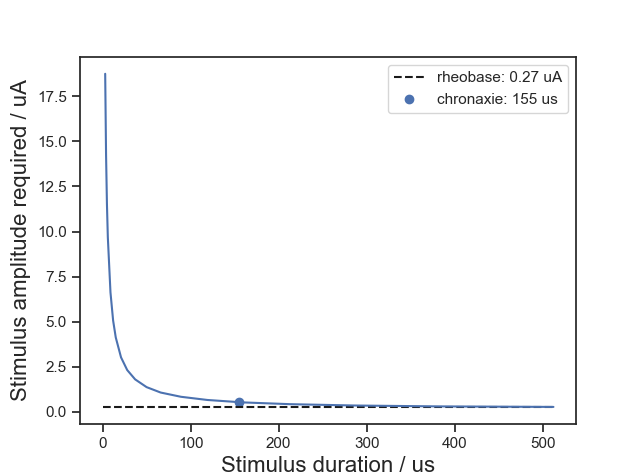
\includegraphics{test_battery_results/Rattay et al. 2001/Strength_duration_curve Rattay et al. 2001.png}
\caption{title}
\end{figure}

    

    \begin{Verbatim}[commandchars=\\\{\}]
{\color{incolor}In [{\color{incolor}81}]:} \PY{n+nb}{print}\PY{p}{(}\PY{n}{strength\PYZus{}duration\PYZus{}data}\PY{p}{)}
\end{Verbatim}


    \begin{Verbatim}[commandchars=\\\{\}]
                  model Van den Honert and Stypulkowski 1984
rheobase (uA)     0.303                                 95.8
chronaxie (us)  155.300                                  247

    \end{Verbatim}

    \subsection{2. Relative spread of
thresholds}\label{relative-spread-of-thresholds}

    \begin{Verbatim}[commandchars=\\\{\}]
{\color{incolor}In [{\color{incolor}82}]:} \PY{n}{md}\PY{p}{(}\PY{l+s+s2}{\PYZdq{}}\PY{l+s+s2}{![title](}\PY{l+s+si}{\PYZpc{}s}\PY{l+s+s2}{)}\PY{l+s+s2}{\PYZdq{}}\PY{o}{\PYZpc{}}\PY{p}{(}\PY{n}{relative\PYZus{}spread\PYZus{}plot\PYZus{}link}\PY{p}{)}\PY{p}{)}
\end{Verbatim}

\texttt{\color{outcolor}Out[{\color{outcolor}82}]:}
    
    \begin{figure}
\centering
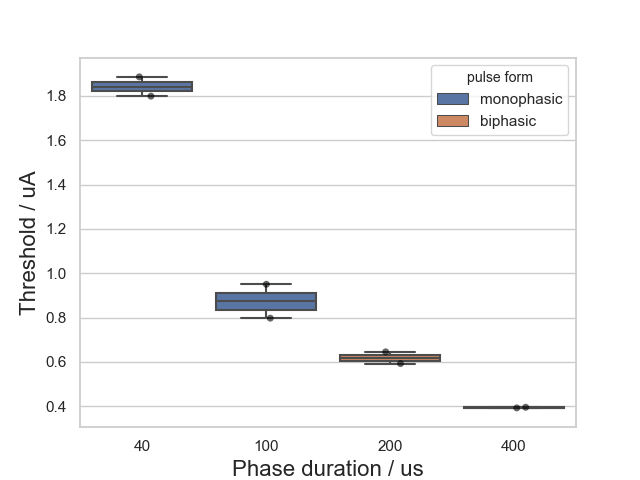
\includegraphics{test_battery_results/Rattay et al. 2001/Relative_spreads_plot Rattay et al. 2001.png}
\caption{title}
\end{figure}

    

    \begin{Verbatim}[commandchars=\\\{\}]
{\color{incolor}In [{\color{incolor}83}]:} \PY{n+nb}{print}\PY{p}{(}\PY{n}{relative\PYZus{}spreads}\PY{p}{)}
\end{Verbatim}


    \begin{Verbatim}[commandchars=\\\{\}]
                            model experiments           reference
phase duration pulse form                                        
40. us         mono         4.41\%        6.3\%  Miller et al. 1999
100. us        mono         10.1\%       5-10\%          Dynes 1996
200. us        bi           8.08\%         12\%   Javel et al. 1987
0.4 ms         bi          10.41\%         11\%   Javel et al. 1987

    \end{Verbatim}

    \subsection{3. Conduction velocity}\label{conduction-velocity}

    \begin{Verbatim}[commandchars=\\\{\}]
{\color{incolor}In [{\color{incolor}84}]:} \PY{n+nb}{print}\PY{p}{(}\PY{n}{conduction\PYZus{}velocity\PYZus{}table}\PY{p}{)}
\end{Verbatim}


    \begin{Verbatim}[commandchars=\\\{\}]
                             model Hursh 1939 Boyd and Kalu 1979           Czèh et al 1976
velocity dendrite (m/s)      6.839          -                  -                         -
velocity/diameter dendrite   4.070          6                4.6                         -
velocity axon (m/s)         12.840          -                  -                         -
velocity/diameter axon       3.820          -                  -  v\_ax = 0.9*v\_den-6.9*m/s

    \end{Verbatim}

    \subsection{4. Single node response
properties}\label{single-node-response-properties}

    \begin{Verbatim}[commandchars=\\\{\}]
{\color{incolor}In [{\color{incolor}85}]:} \PY{n}{md}\PY{p}{(}\PY{l+s+s2}{\PYZdq{}}\PY{l+s+s2}{![title](}\PY{l+s+si}{\PYZpc{}s}\PY{l+s+s2}{)}\PY{l+s+s2}{\PYZdq{}}\PY{o}{\PYZpc{}}\PY{p}{(}\PY{n}{single\PYZus{}node\PYZus{}response\PYZus{}link}\PY{p}{)}\PY{p}{)}
\end{Verbatim}

\texttt{\color{outcolor}Out[{\color{outcolor}85}]:}
    
    \begin{figure}
\centering
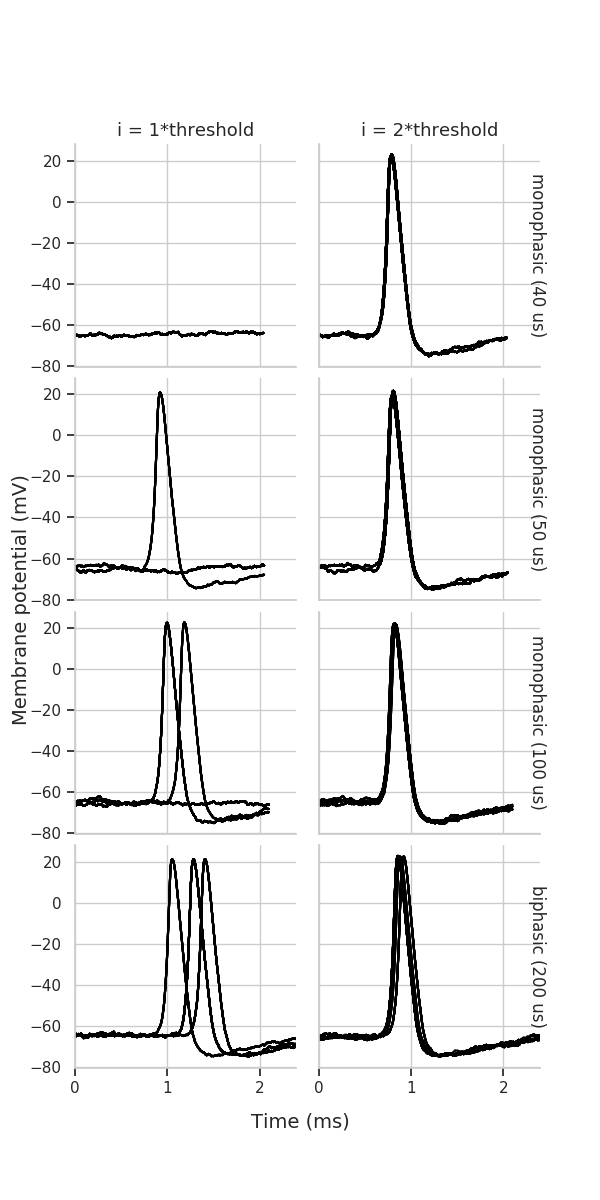
\includegraphics{test_battery_results/Rattay et al. 2001/Single_node_response Rattay et al. 2001.png}
\caption{title}
\end{figure}

    

    \subsubsection{4.1 Action potential shape}\label{action-potential-shape}

    \begin{Verbatim}[commandchars=\\\{\}]
{\color{incolor}In [{\color{incolor}86}]:} \PY{n+nb}{print}\PY{p}{(}\PY{n}{AP\PYZus{}shape}\PY{p}{)}
\end{Verbatim}


    \begin{Verbatim}[commandchars=\\\{\}]
                   model Paintal 1965
AP height (mV)    87.200            -
rise time (ms)     0.110        0.136
fall time (ms)     0.196        0.379
AP duration (ms)   0.307        0.515

    \end{Verbatim}

    \subsubsection{4.2 Latency and jitter}\label{latency-and-jitter}

    \begin{Verbatim}[commandchars=\\\{\}]
{\color{incolor}In [{\color{incolor}87}]:} \PY{n+nb}{print}\PY{p}{(}\PY{n}{latency\PYZus{}jitter}\PY{p}{)}
\end{Verbatim}


    \begin{Verbatim}[commandchars=\\\{\}]
                                             model (threshold)  model (2*threshold) Miller et al. 1999  \textbackslash{}
phase duration (us) pulse form variable                                                                  
40.0                monophasic latency (us)              533.3                 99.0                650   
                               jitter (us)               128.8                  3.2                100   
50.0                monophasic latency (us)              552.0                109.0                  -   
                               jitter (us)                41.6                  3.2                  -   
100.0               monophasic latency (us)              460.0                141.5                  -   
                               jitter (us)                76.0                  3.4                  -   
200.0               biphasic   latency (us)              483.0                183.5                  -   
                               jitter (us)               107.4                  4.7                  -   

                                            Van den Honert and Stypulkowski 1984 (threshold)  \textbackslash{}
phase duration (us) pulse form variable                                                        
40.0                monophasic latency (us)                                                -   
                               jitter (us)                                                 -   
50.0                monophasic latency (us)                                                -   
                               jitter (us)                                                 -   
100.0               monophasic latency (us)                                              685   
                               jitter (us)                                               352   
200.0               biphasic   latency (us)                                                -   
                               jitter (us)                                                 -   

                                            Van den Honert and Stypulkowski 1984 (2*threshold)  \textbackslash{}
phase duration (us) pulse form variable                                                          
40.0                monophasic latency (us)                                                  -   
                               jitter (us)                                                   -   
50.0                monophasic latency (us)                                                  -   
                               jitter (us)                                                   -   
100.0               monophasic latency (us)                                                352   
                               jitter (us)                                                   8   
200.0               biphasic   latency (us)                                                  -   
                               jitter (us)                                                   -   

                                            Hartmann and al. 1984 Cartee et al. 2000 (threshold)  
phase duration (us) pulse form variable                                                           
40.0                monophasic latency (us)                     -                              -  
                               jitter (us)                      -                              -  
50.0                monophasic latency (us)                     -                            440  
                               jitter (us)                      -                             80  
100.0               monophasic latency (us)                     -                              -  
                               jitter (us)                      -                              -  
200.0               biphasic   latency (us)               300-400                              -  
                               jitter (us)                      -                              -  

    \end{Verbatim}

    \subsection{5. Recfractory properties}\label{recfractory-properties}

    \begin{Verbatim}[commandchars=\\\{\}]
{\color{incolor}In [{\color{incolor}88}]:} \PY{n}{md}\PY{p}{(}\PY{l+s+s2}{\PYZdq{}}\PY{l+s+s2}{![title](}\PY{l+s+si}{\PYZpc{}s}\PY{l+s+s2}{)}\PY{l+s+s2}{\PYZdq{}}\PY{o}{\PYZpc{}}\PY{p}{(}\PY{n}{refractory\PYZus{}curve\PYZus{}link}\PY{p}{)}\PY{p}{)}
\end{Verbatim}

\texttt{\color{outcolor}Out[{\color{outcolor}88}]:}
    
    \begin{figure}
\centering
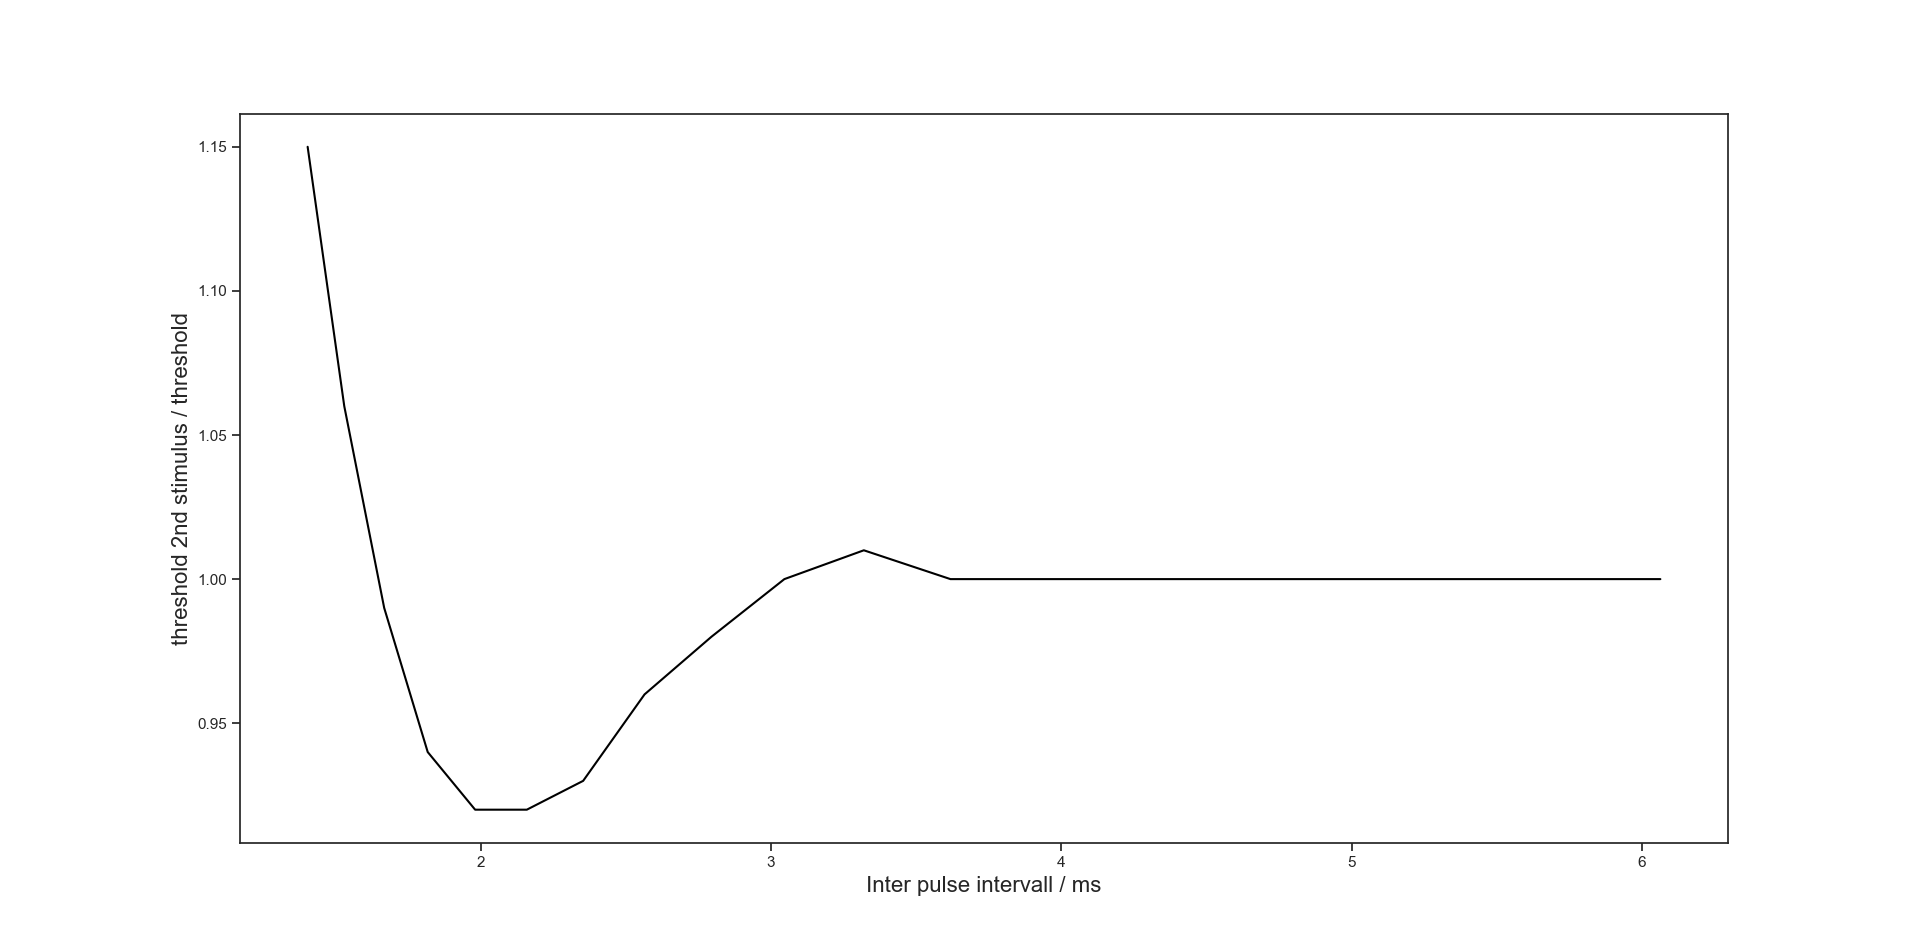
\includegraphics{test_battery_results/Rattay et al. 2001/Refractory_curve Rattay et al. 2001.png}
\caption{title}
\end{figure}

    

    \subsubsection{5.1 Absolute refractory
periods}\label{absolute-refractory-periods}

    \begin{Verbatim}[commandchars=\\\{\}]
{\color{incolor}In [{\color{incolor}89}]:} \PY{n+nb}{print}\PY{p}{(}\PY{n}{absolute\PYZus{}refractory\PYZus{}periods}\PY{p}{)}
\end{Verbatim}


    \begin{Verbatim}[commandchars=\\\{\}]
                                ARP model (us) ARP Experiments (us)                             reference
phase duration (us) pulse form                                                                           
40.0                monophasic          1393.0                  334                    Miller et al. 2001
50.0                monophasic          1393.0                  300  Stypulkowski and Van den Honert 1984
100.0               monophasic          1353.0              500-700                            Dynes 1996
50.0                biphasic            1383.0              400-500                  Brown and Abbas 1990

    \end{Verbatim}

    \subsubsection{5.2 Relative refractory
periods}\label{relative-refractory-periods}

    \begin{Verbatim}[commandchars=\\\{\}]
{\color{incolor}In [{\color{incolor}90}]:} \PY{n+nb}{print}\PY{p}{(}\PY{n}{relative\PYZus{}refractory\PYZus{}periods}\PY{p}{)}
\end{Verbatim}


    \begin{Verbatim}[commandchars=\\\{\}]
                                RRP model (ms) RRP Experiments (ms)  \textbackslash{}
phase duration (us) pulse form                                        
50.0                monophasic           1.478             3-4; 4-5   
100.0               monophasic           1.468                    5   
200.0               biphasic             1.188                    5   

                                                                        reference  
phase duration (us) pulse form                                                     
50.0                monophasic  Stypulkowski and Van den Honert 1984; Cartee e{\ldots}  
100.0               monophasic                                         Dynes 1996  
200.0               biphasic                                 Hartmann et al. 1984  

    \end{Verbatim}

    \subsection{6. Post-stimulus time
histogramm}\label{post-stimulus-time-histogramm}

    \begin{Verbatim}[commandchars=\\\{\}]
{\color{incolor}In [{\color{incolor}91}]:} \PY{n}{md}\PY{p}{(}\PY{l+s+s2}{\PYZdq{}}\PY{l+s+s2}{![title](}\PY{l+s+si}{\PYZpc{}s}\PY{l+s+s2}{)}\PY{l+s+s2}{\PYZdq{}}\PY{o}{\PYZpc{}}\PY{p}{(}\PY{n}{post\PYZus{}stimulus\PYZus{}time\PYZus{}histogram\PYZus{}link}\PY{p}{)}\PY{p}{)}
\end{Verbatim}

\texttt{\color{outcolor}Out[{\color{outcolor}91}]:}
    
    \begin{figure}
\centering
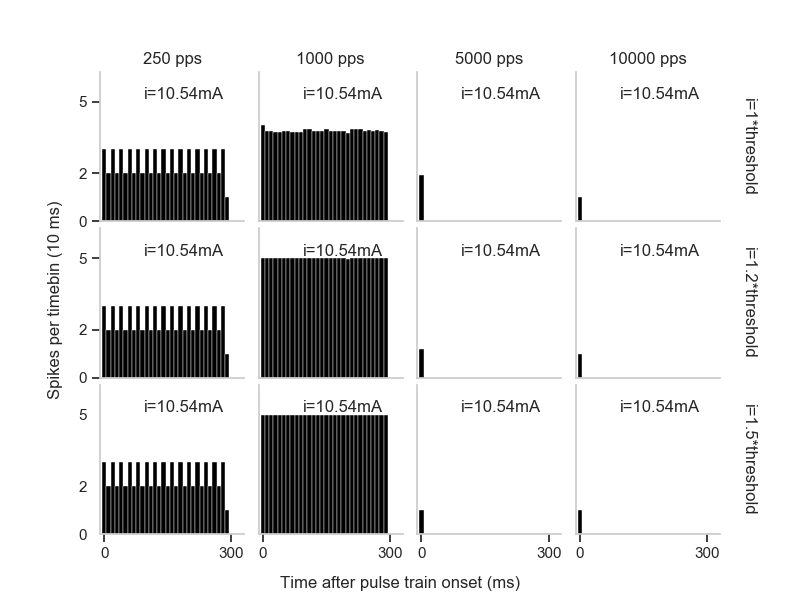
\includegraphics{test_battery_results/Rattay et al. 2001/PSTH Rattay et al. 2001.png}
\caption{title}
\end{figure}

    


    % Add a bibliography block to the postdoc
    
    
    
    \end{document}
